\clearpage
\section{Supplementary Diagnostics}
\label{app:skewness}
This appendix gathers additional descriptive material used in the preprocessing discussion.

\subsection{Mean-to-Median Ratio}
\label{subsec:mean_ratio}
\begin{figure}[H]
\centering
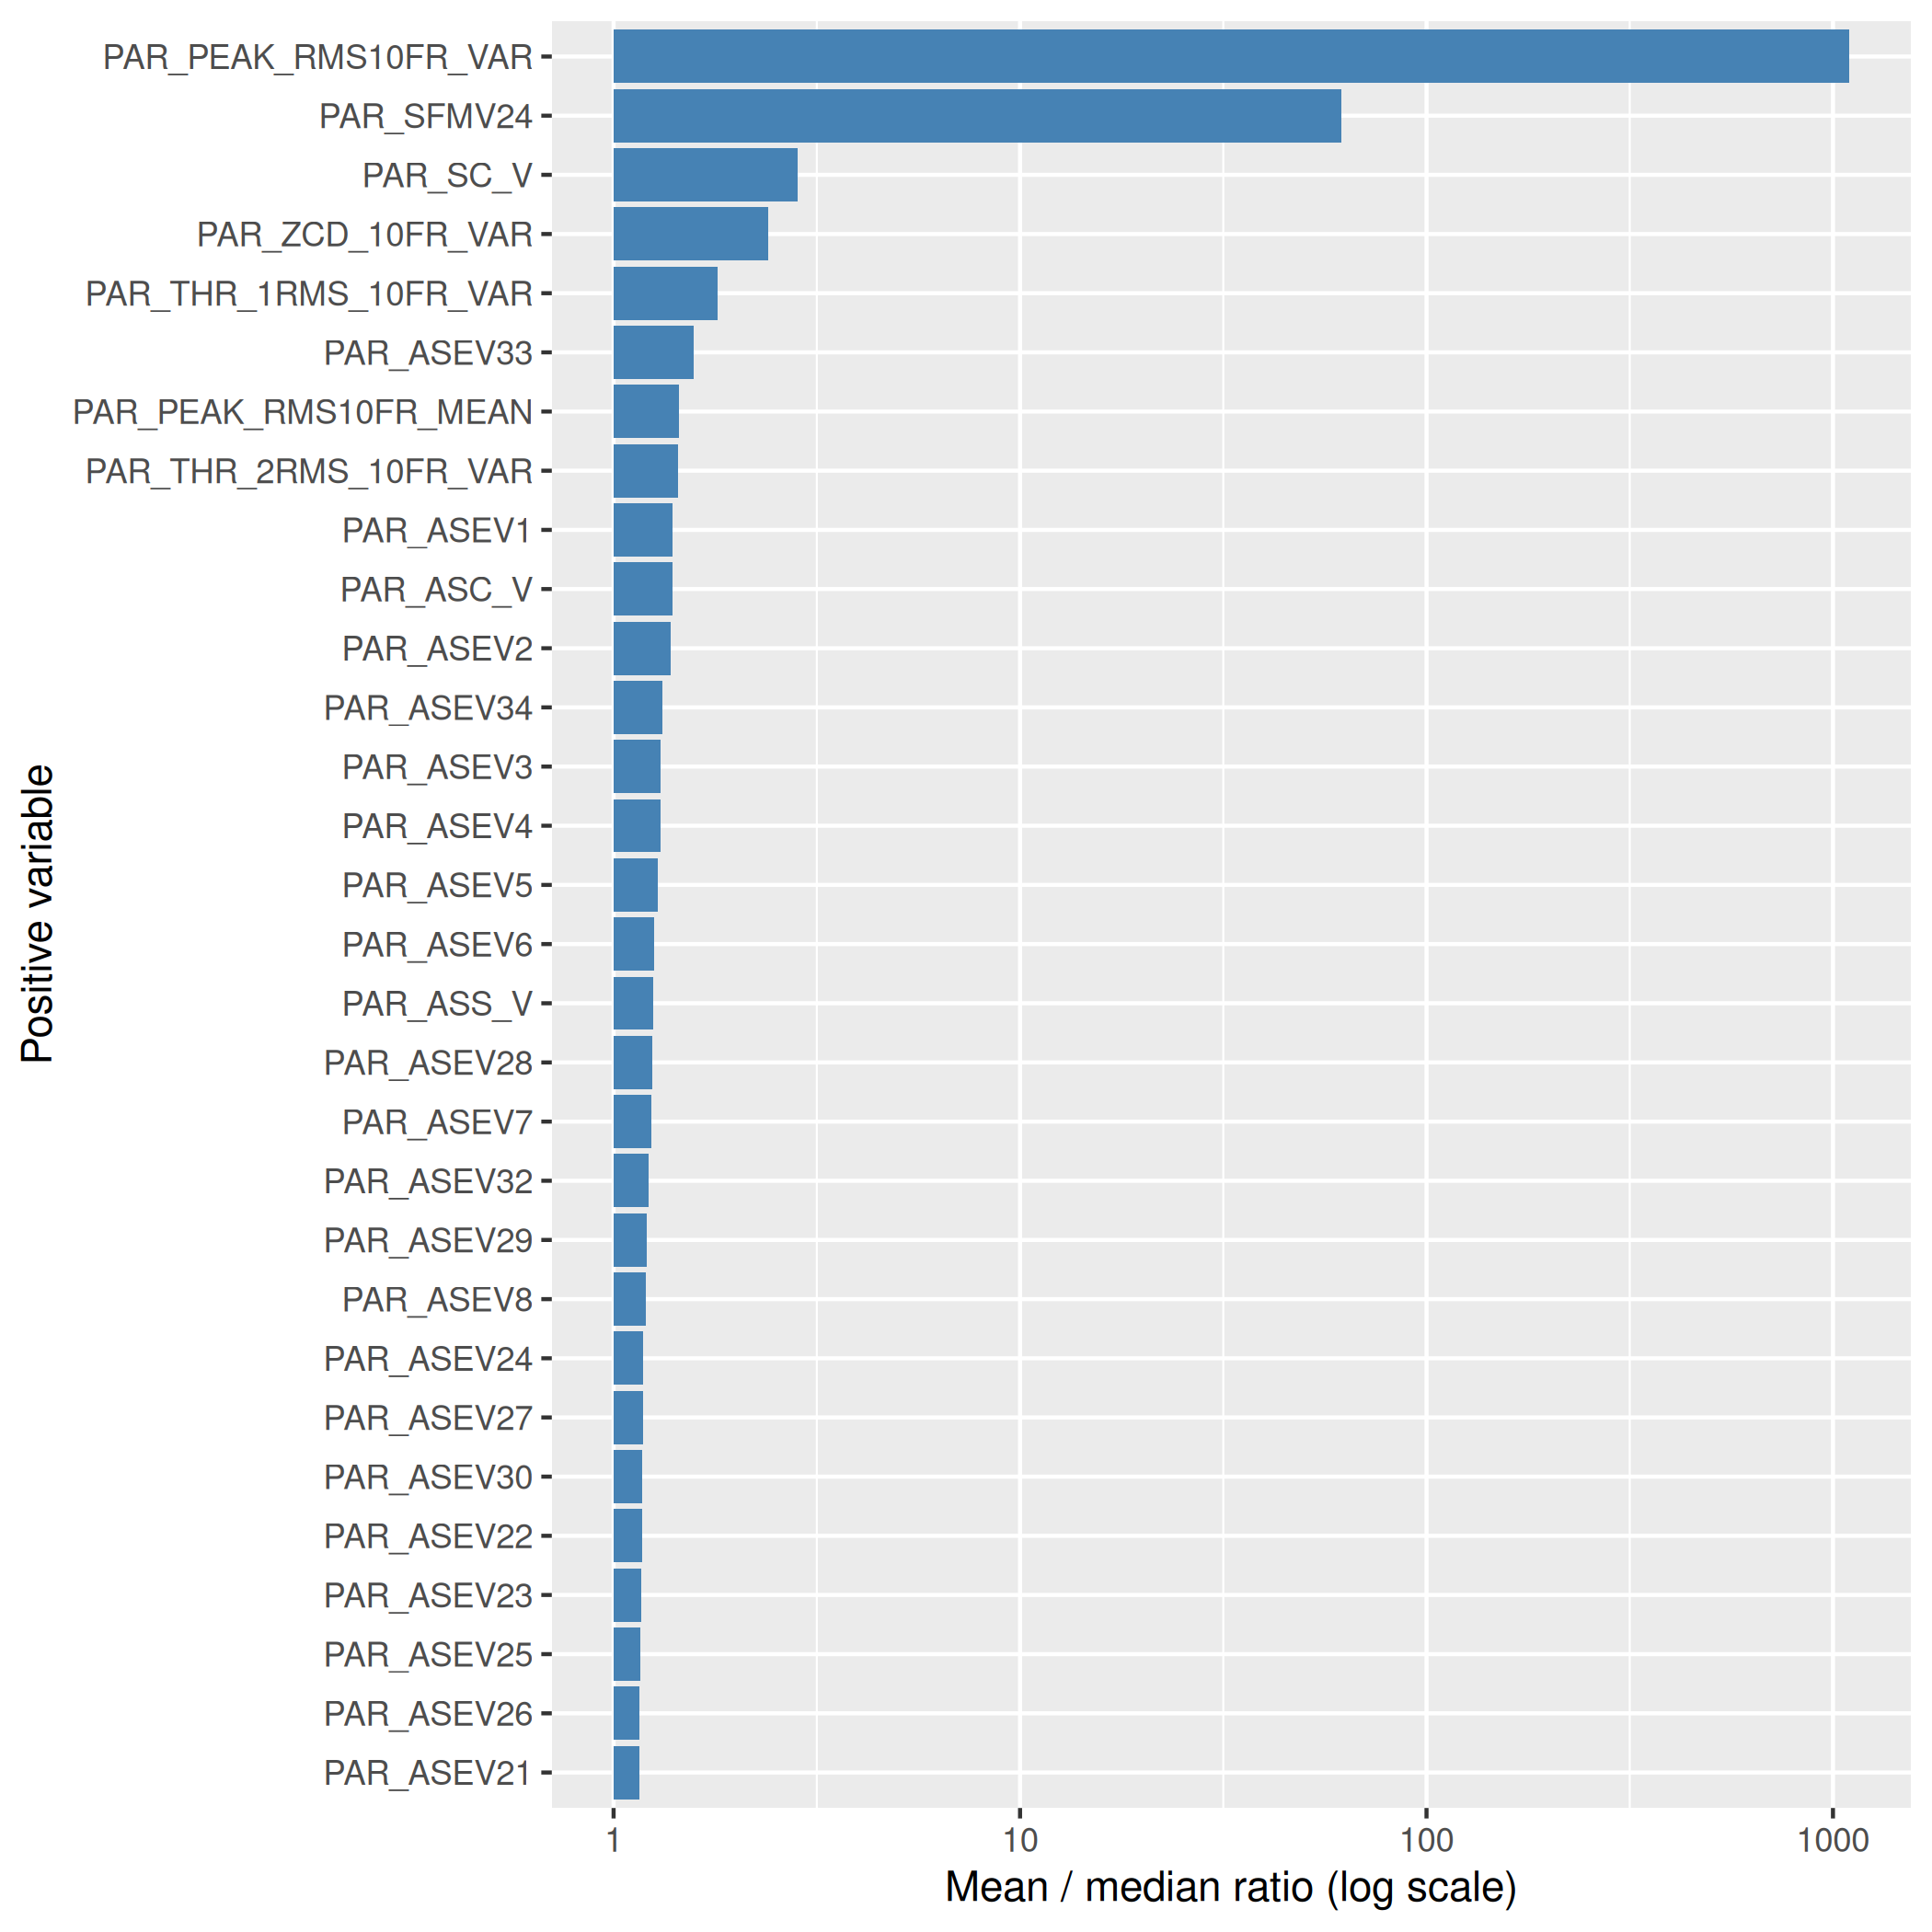
\includegraphics[width=0.78\columnwidth]{../output/part1/log_candidates_mean_median_ratio.png}
\caption{Mean-to-median ratio for the positive variables considered as candidates for a logarithmic transformation. Larger values indicate stronger right-skewness.}
\label{fig:mean_ratio}
\end{figure}

\subsection{Skewness}
\label{subsec:skewness}
The skewness coefficient used in the report follows the standardized third central moment given by NIST/SEMATECH~\cite{nistskewness}:
\begin{equation}
g_{1}=\frac{\frac{1}{N}\sum_{i=1}^{N}(Y_{i}-\bar{Y})^{3}}{s^{3}},
\label{eq:skewness}
\end{equation}
where \(\bar{Y}\) is the sample mean and \(s\) is the sample standard deviation. Positive values indicate right-skewness, negative values indicate left-skewness, and values close to zero correspond to more symmetric distributions.

\begin{figure}[H]
\centering
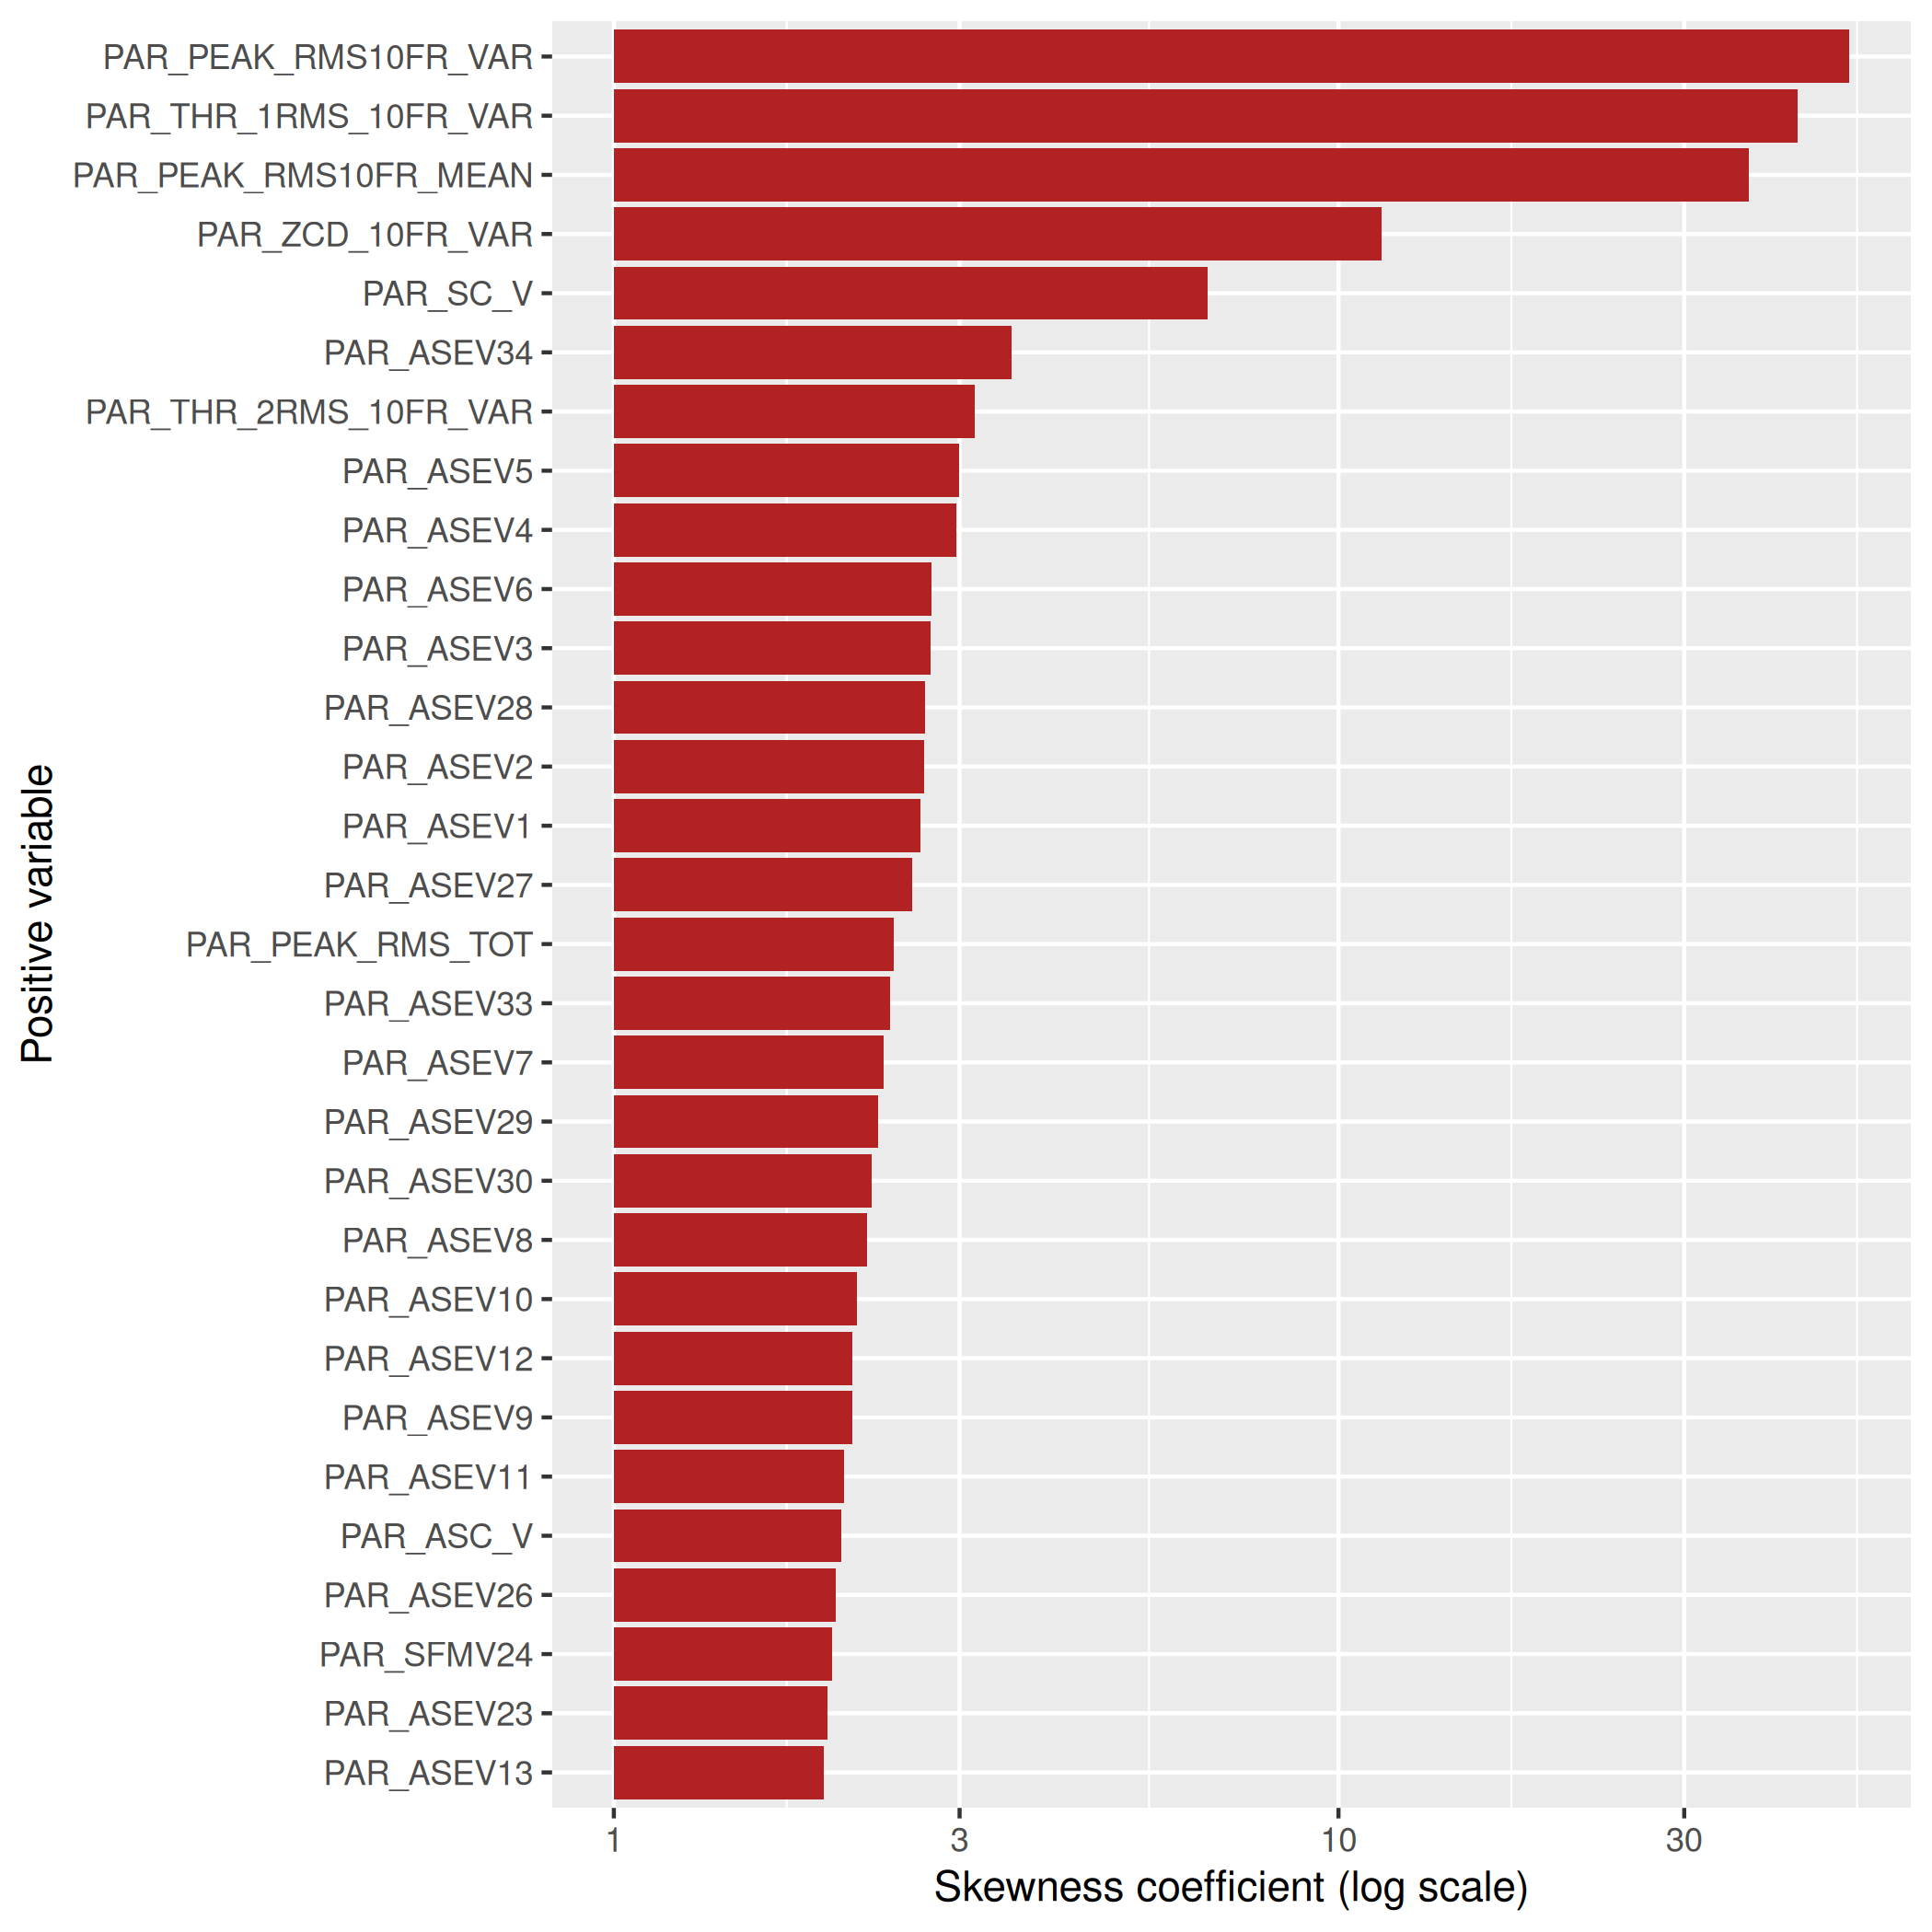
\includegraphics[width=0.78\columnwidth]{../output/part1/log_candidates_skewness.png}
\caption{Sample skewness for the variables considered as candidates for a logarithmic transformation. Larger positive values indicate stronger right-skewness.}
\label{fig:skewness_candidates}
\end{figure}

\subsection{Heteroscedasticity}
\label{subsec:heteroscedasticity}
Heteroscedasticity is important in the present analysis because, even when a variable is strongly right-skewed, a logarithmic transformation is especially relevant when the dispersion also tends to increase with the level of the measurements. Van den Berg et al.~\cite{vandenberg2006preprocessing} note that logarithmic transformations are used in part to stabilize spread, while the NIST/SEMATECH \emph{spread-location} diagnostic emphasizes the practical importance of examining how variability changes with location \cite{nistspreadlocation}. Following this idea, the implemented score is a descriptive screening tool: each strictly positive variable is partitioned into \(K=10\) empirical-quantile groups, the group means \(\bar{X}_g\) and group standard deviations \(s_g\) are computed, and the monotone association between level and spread is summarized by Spearman's rank correlation \cite{nistrankcorrelation},
\begin{equation}
H(X)=\rho_S\!\left((\bar{X}_g)_{g \in \mathcal{G}},(s_g)_{g \in \mathcal{G}}\right),
\label{eq:heteroscedasticity_score_app}
\end{equation}
where \(\rho_S\) is Spearman's coefficient and \(\mathcal{G}\) denotes the set of groups for which both summaries are finite. Large positive values of \(H(X)\) indicate a clear \emph{spread-versus-level} pattern, meaning that higher average values are associated with higher within-group dispersion; for that reason, this score is used together with the mean-to-median ratio and skewness to identify plausible candidates for a logarithmic transformation. The corresponding ranking of variables is shown in Fig.~\ref{fig:heteroscedasticity_candidates}.

\begin{figure}[H]
\centering
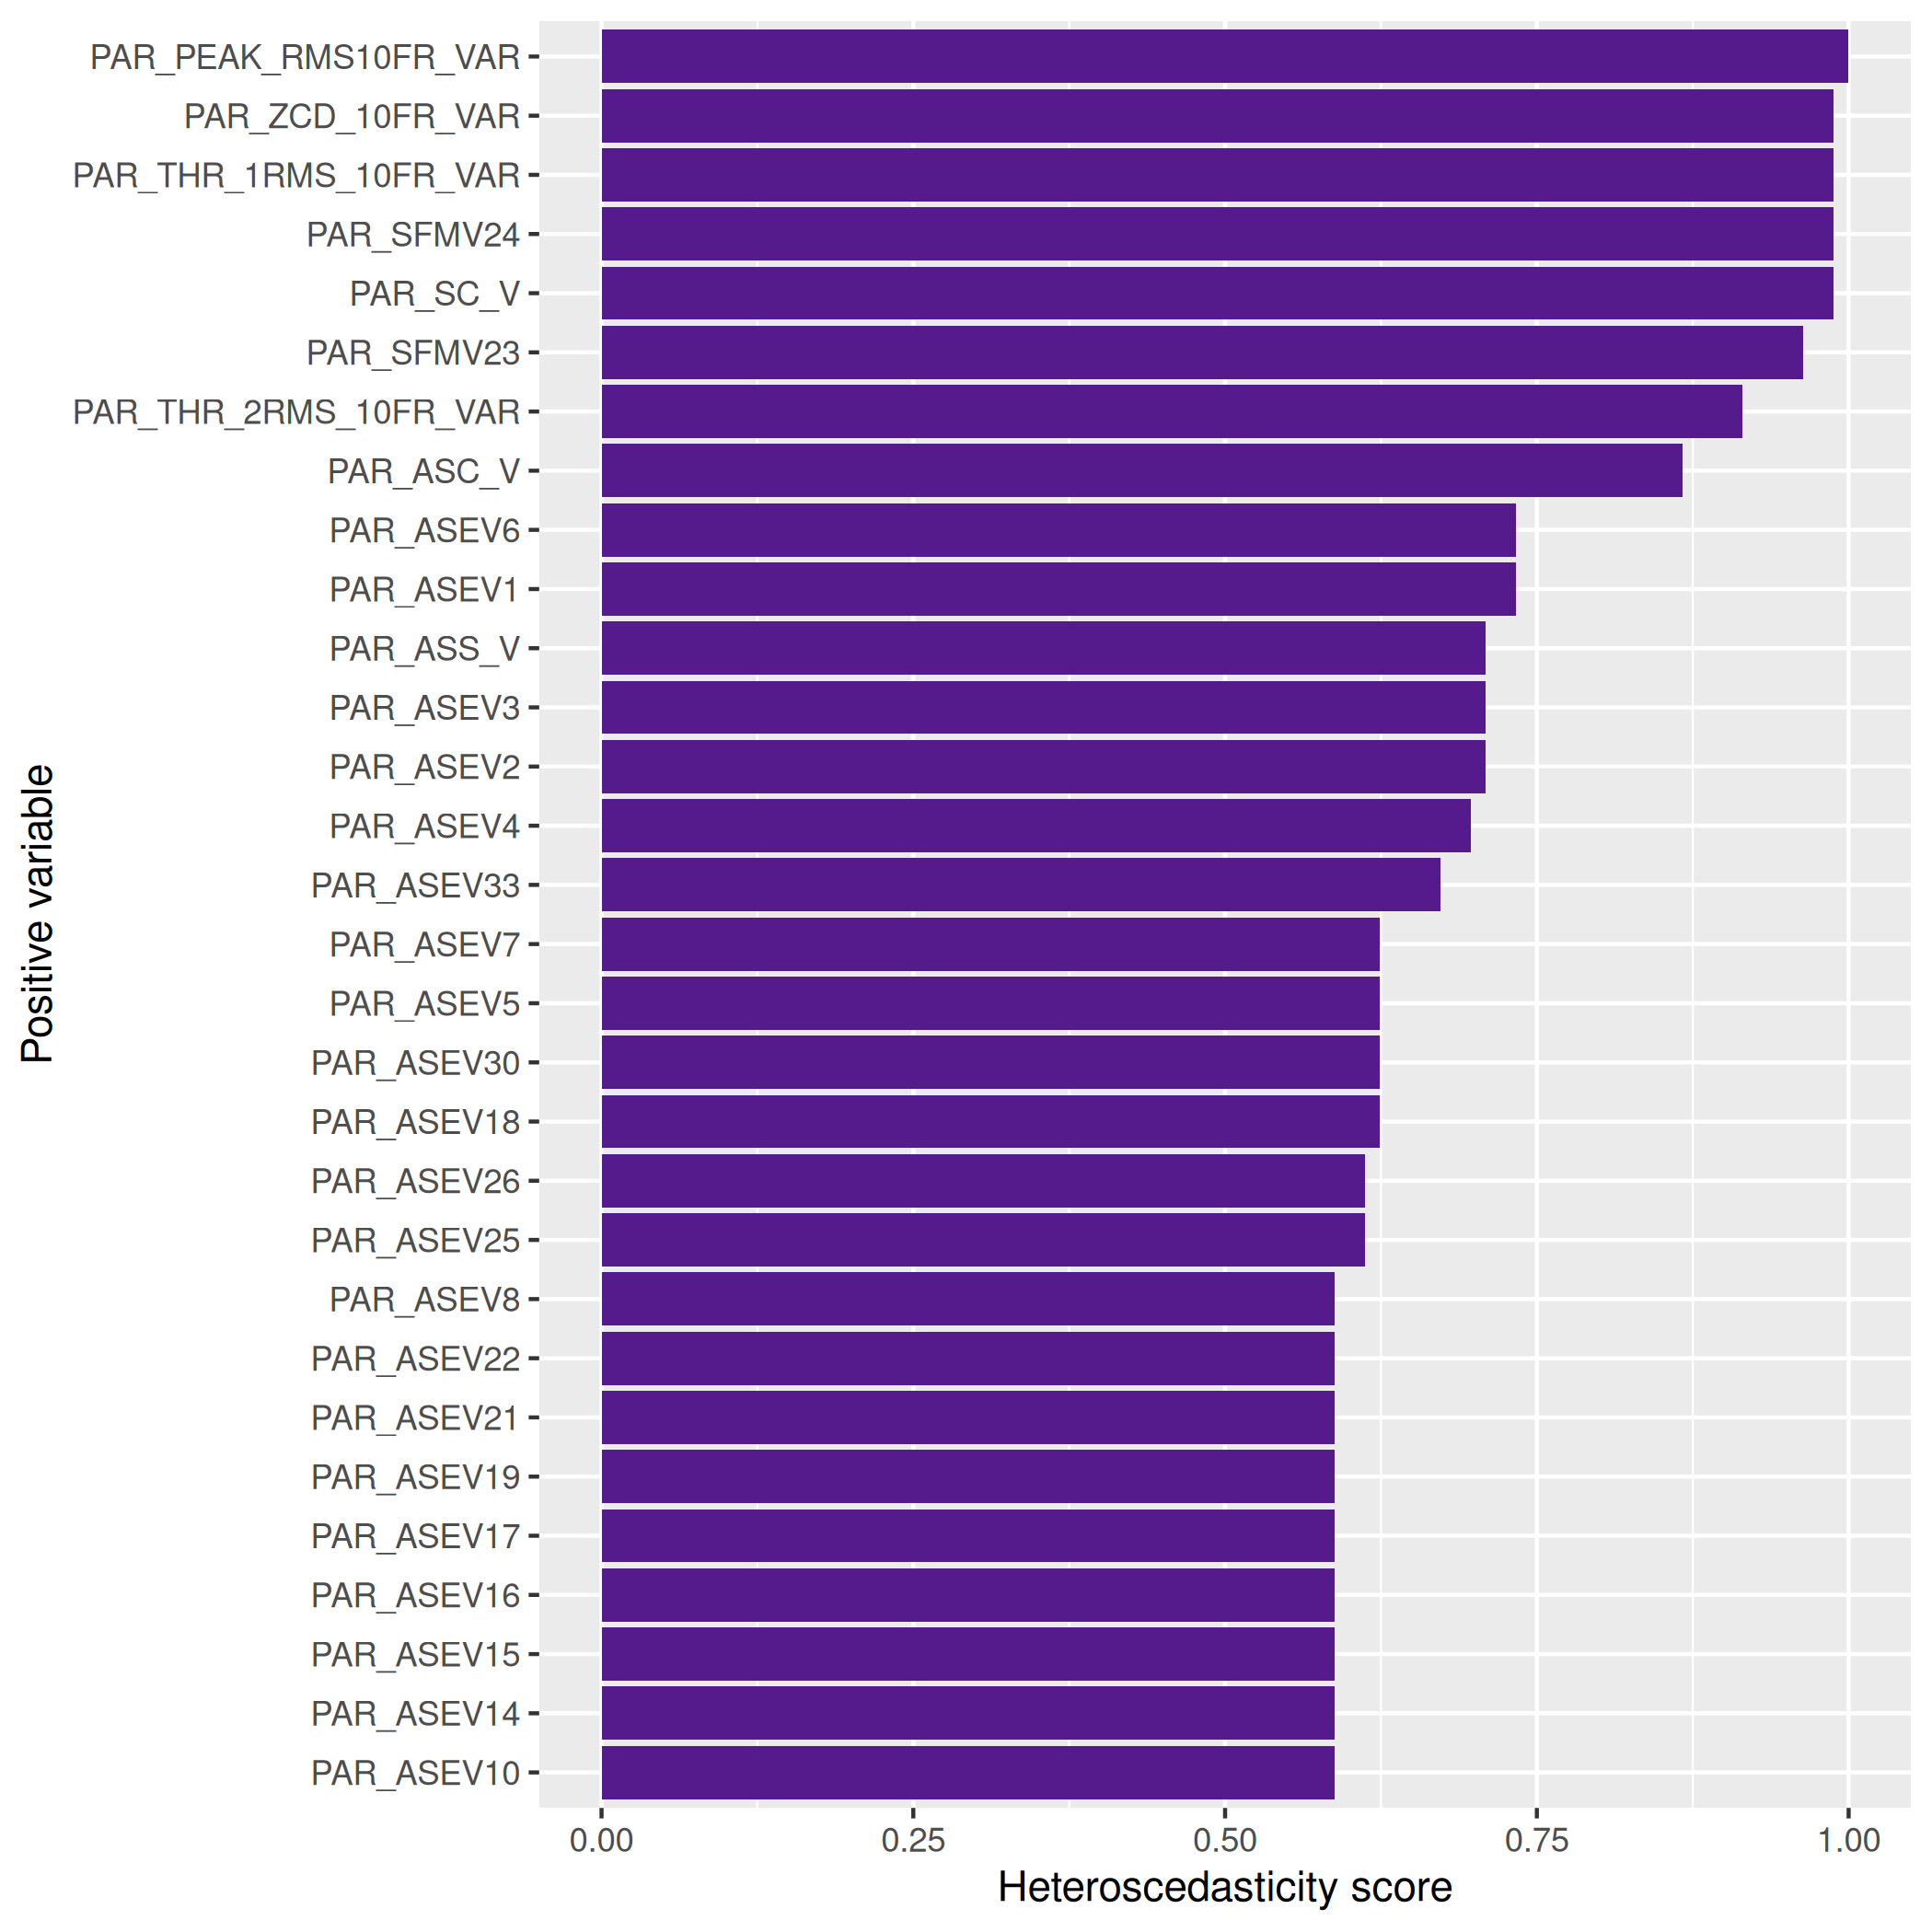
\includegraphics[width=0.78\columnwidth]{../output/part1/log_candidates_heteroscedasticity.png}
\caption{Heteroscedasticity score for the positive variables considered as candidates for a logarithmic transformation. Larger positive values indicate a stronger spread-versus-level pattern.}
\label{fig:heteroscedasticity_candidates}
\end{figure}

\subsection{Log-Normality}
\label{subsec:log_normality}
For the variables retained simultaneously by the asymmetry and heteroscedasticity screens, we finally examine whether the logarithmic transformation produces a distribution closer to normality. The set of common candidate variables is listed in Table~\ref{tab:common_candidates}. We then apply the Shapiro--Wilk test to \(\log(X)\) and rank these variables by the resulting \(W\) statistic, where values closer to \(1\) indicate a better agreement with normality. In basic terms, the \texttt{variable} column gives the name of the candidate predictor, \texttt{shapiro\_w} is the Shapiro--Wilk statistic computed on \(\log(X)\), and \texttt{p\_value} is the corresponding significance level for the null hypothesis that \(\log(X)\) is normally distributed. The values reported in Table~\ref{tab:log_normality_candidates} are obtained by applying the test to each positive variable that was retained by the previous screening criteria.

\begin{table}[H]
\centering
\caption{Variables retained simultaneously by the asymmetry and heteroscedasticity screening criteria.}
\label{tab:common_candidates}
\scriptsize
\begin{tabular}{rl}
\toprule
\# & Variable \\
\midrule
1 & PAR\_PEAK\_RMS10FR\_VAR \\
2 & PAR\_SFMV24 \\
3 & PAR\_SC\_V \\
4 & PAR\_ZCD\_10FR\_VAR \\
5 & PAR\_THR\_1RMS\_10FR\_VAR \\
6 & PAR\_ASEV33 \\
7 & PAR\_THR\_2RMS\_10FR\_VAR \\
8 & PAR\_ASEV1 \\
9 & PAR\_ASC\_V \\
10 & PAR\_ASEV2 \\
11 & PAR\_ASEV3 \\
12 & PAR\_ASEV4 \\
13 & PAR\_ASEV5 \\
14 & PAR\_ASEV6 \\
15 & PAR\_ASEV7 \\
16 & PAR\_ASEV8 \\
17 & PAR\_ASEV30 \\
18 & PAR\_ASEV26 \\
\bottomrule
\end{tabular}
\end{table}

\begin{figure}[H]
\centering
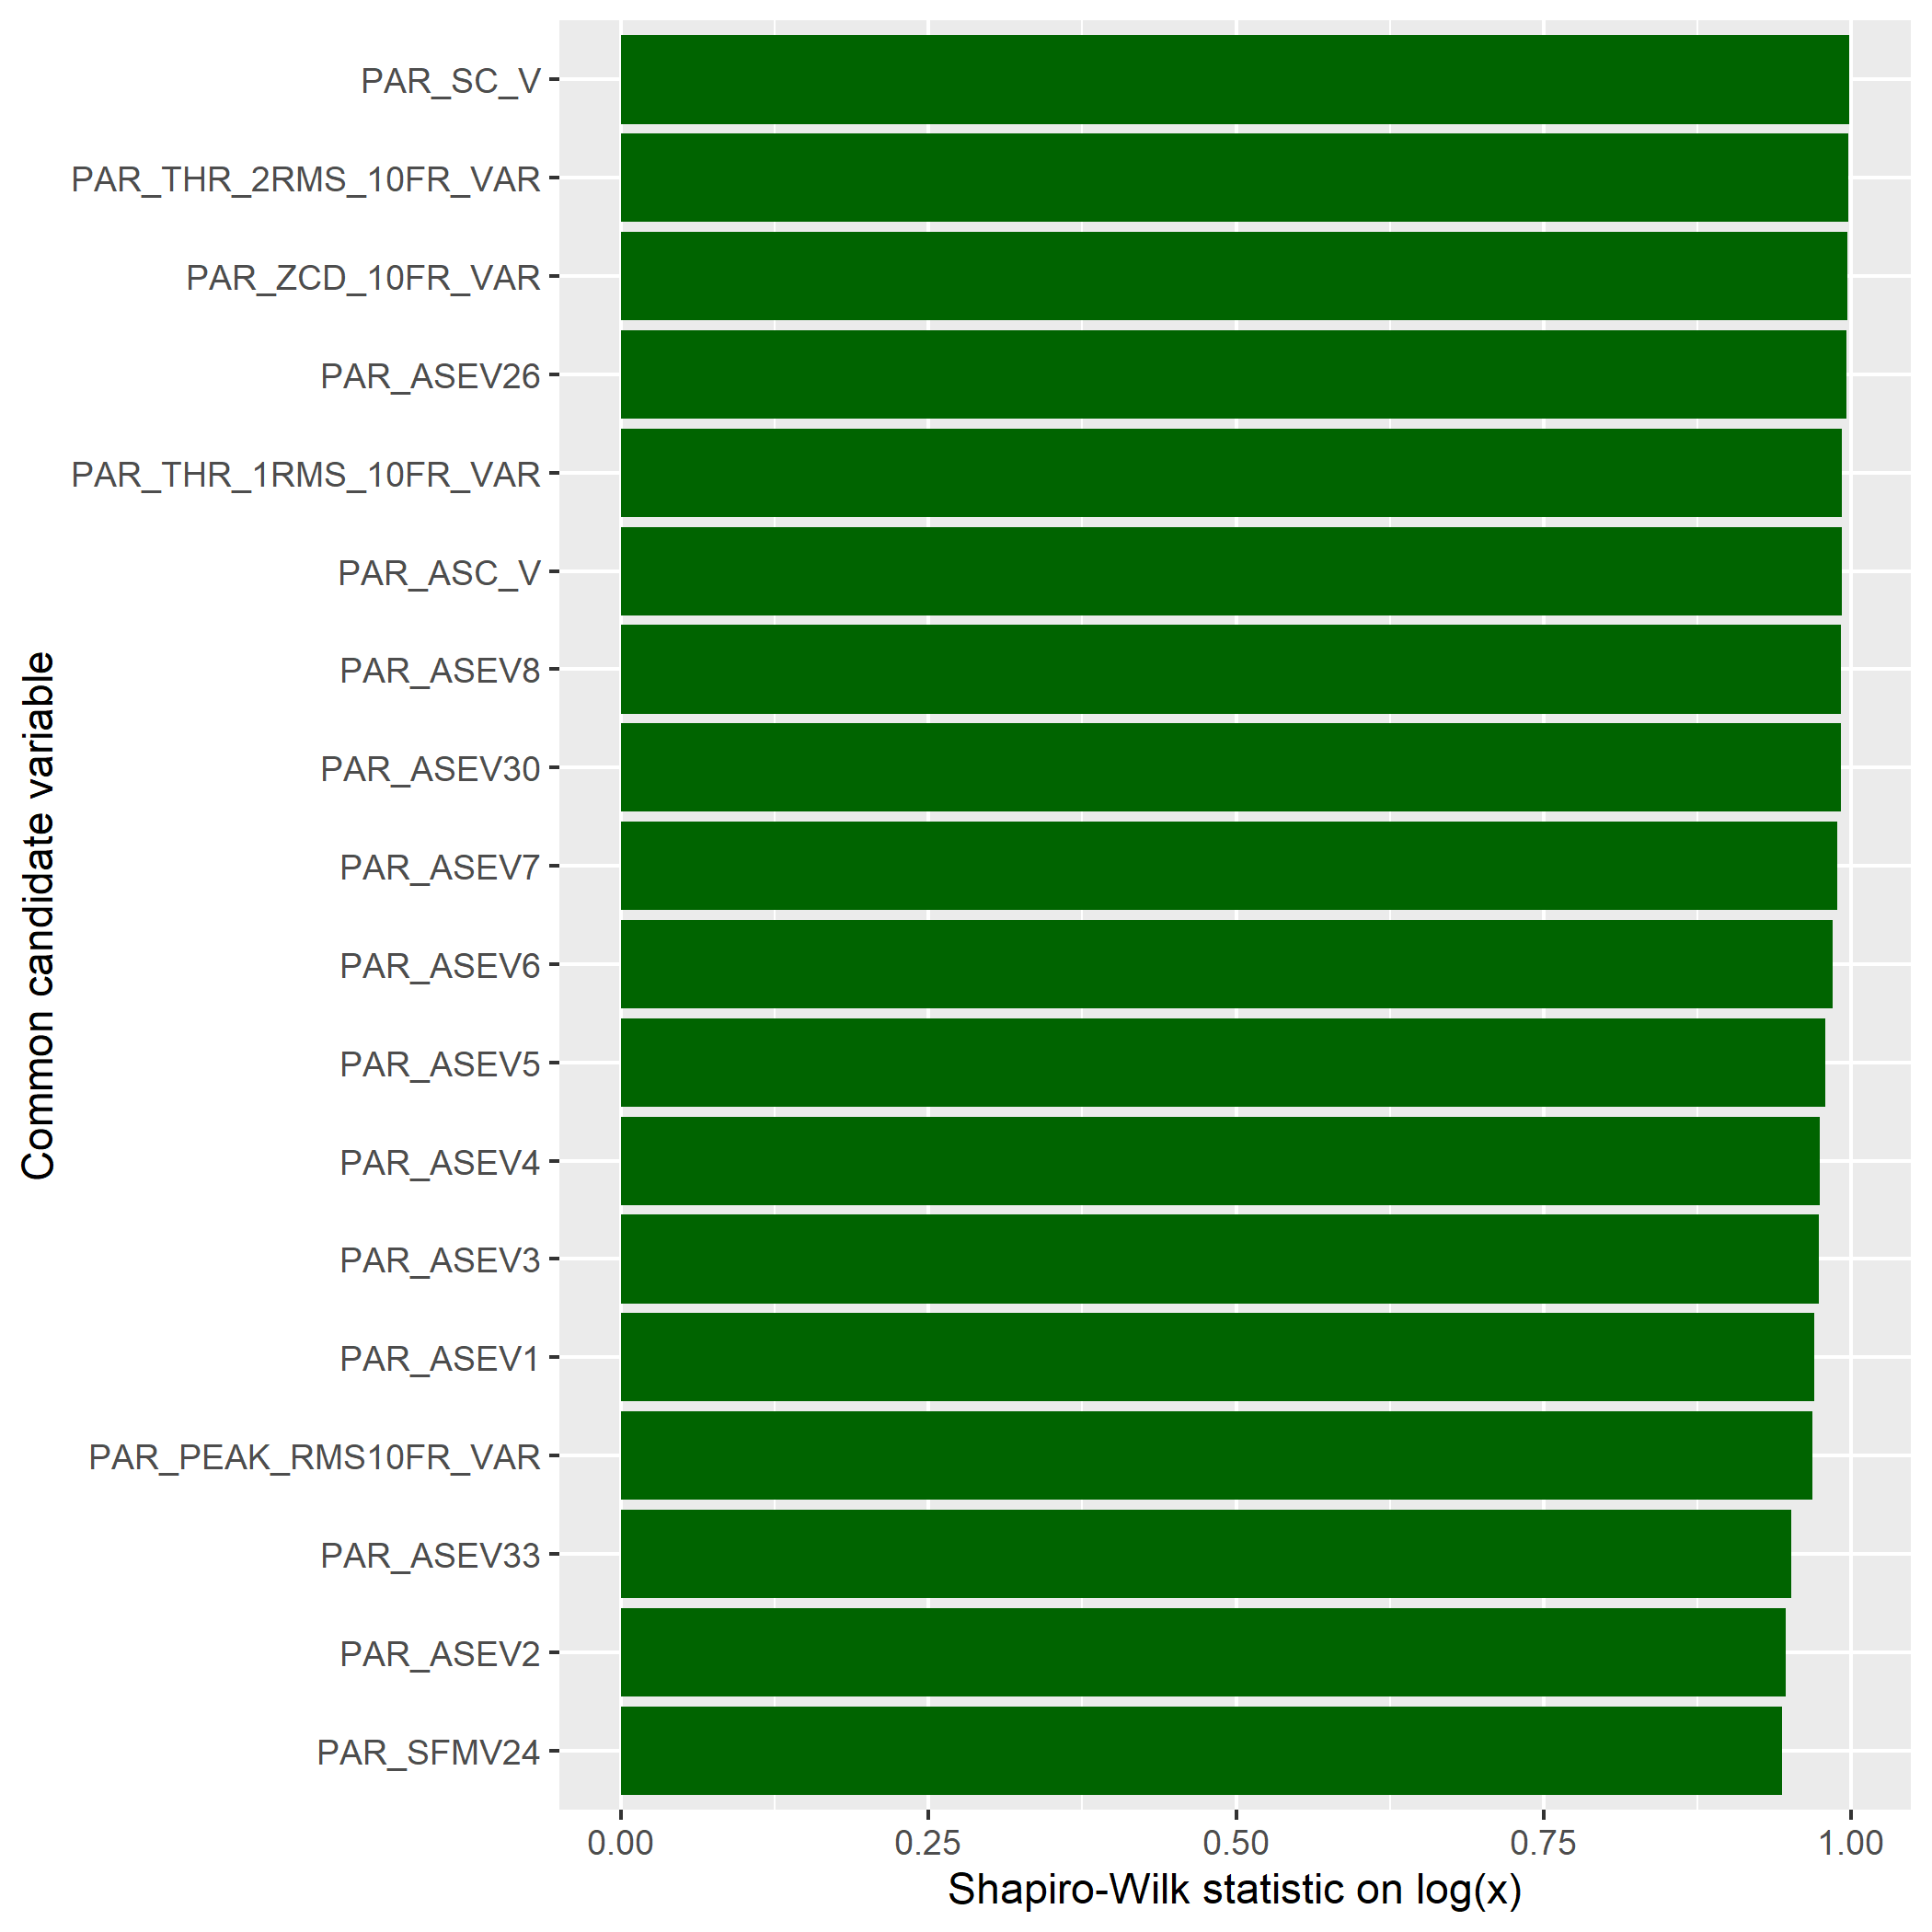
\includegraphics[width=0.78\columnwidth]{../output/part1/common_candidates_log_normality.png}
\caption{Shapiro--Wilk \(W\) statistic computed on \(\log(X)\) for the common candidate variables. Larger values indicate that the log-transformed variable is closer to a normal distribution.}
\label{fig:log_normality_candidates}
\end{figure}

\begin{table}[H]
\centering
\caption{Shapiro--Wilk results on \(\log(X)\) for the common candidate variables.}
\label{tab:log_normality_candidates}
\scriptsize
\begin{tabular}{lll}
\toprule
Variable & \(\boldsymbol{W}\) & \(\boldsymbol{p}\)-value \\
\midrule
PAR\_SC\_V & 0.9984029 & \(6.06 \times 10^{-5}\) \\
PAR\_THR\_2RMS\_10FR\_VAR & 0.9977017 & \(7.98 \times 10^{-7}\) \\
PAR\_ZCD\_10FR\_VAR & 0.9969759 & \(1.70 \times 10^{-8}\) \\
PAR\_ASEV26 & 0.9961615 & \(4.01 \times 10^{-10}\) \\
PAR\_THR\_1RMS\_10FR\_VAR & 0.9922652 & \(7.13 \times 10^{-16}\) \\
PAR\_ASC\_V & 0.9922296 & \(6.47 \times 10^{-16}\) \\
PAR\_ASEV8 & 0.9916860 & \(1.51 \times 10^{-16}\) \\
PAR\_ASEV30 & 0.9913730 & \(6.72 \times 10^{-17}\) \\
PAR\_ASEV7 & 0.9888169 & \(1.77 \times 10^{-19}\) \\
PAR\_ASEV6 & 0.9853344 & \(2.19 \times 10^{-22}\) \\
PAR\_ASEV5 & 0.9790100 & \(1.45 \times 10^{-26}\) \\
PAR\_ASEV4 & 0.9746038 & \(6.10 \times 10^{-29}\) \\
PAR\_ASEV3 & 0.9737920 & \(2.41 \times 10^{-29}\) \\
PAR\_ASEV1 & 0.9698754 & \(3.67 \times 10^{-31}\) \\
PAR\_PEAK\_RMS10FR\_VAR & 0.9688232 & \(1.28 \times 10^{-31}\) \\
PAR\_ASEV33 & 0.9510785 & \(6.11 \times 10^{-38}\) \\
PAR\_ASEV2 & 0.9469831 & \(3.93 \times 10^{-39}\) \\
PAR\_SFMV24 & 0.9436739 & \(4.84 \times 10^{-40}\) \\
\bottomrule
\end{tabular}
\end{table}

\subsection{PCA Variable Space}
\label{subsec:pca_variable_space}
The following tables summarize the main diagnostics used to interpret the variable space of the PCA after preprocessing and standardization of the 165 retained predictors.

\begin{figure}[H]
\centering
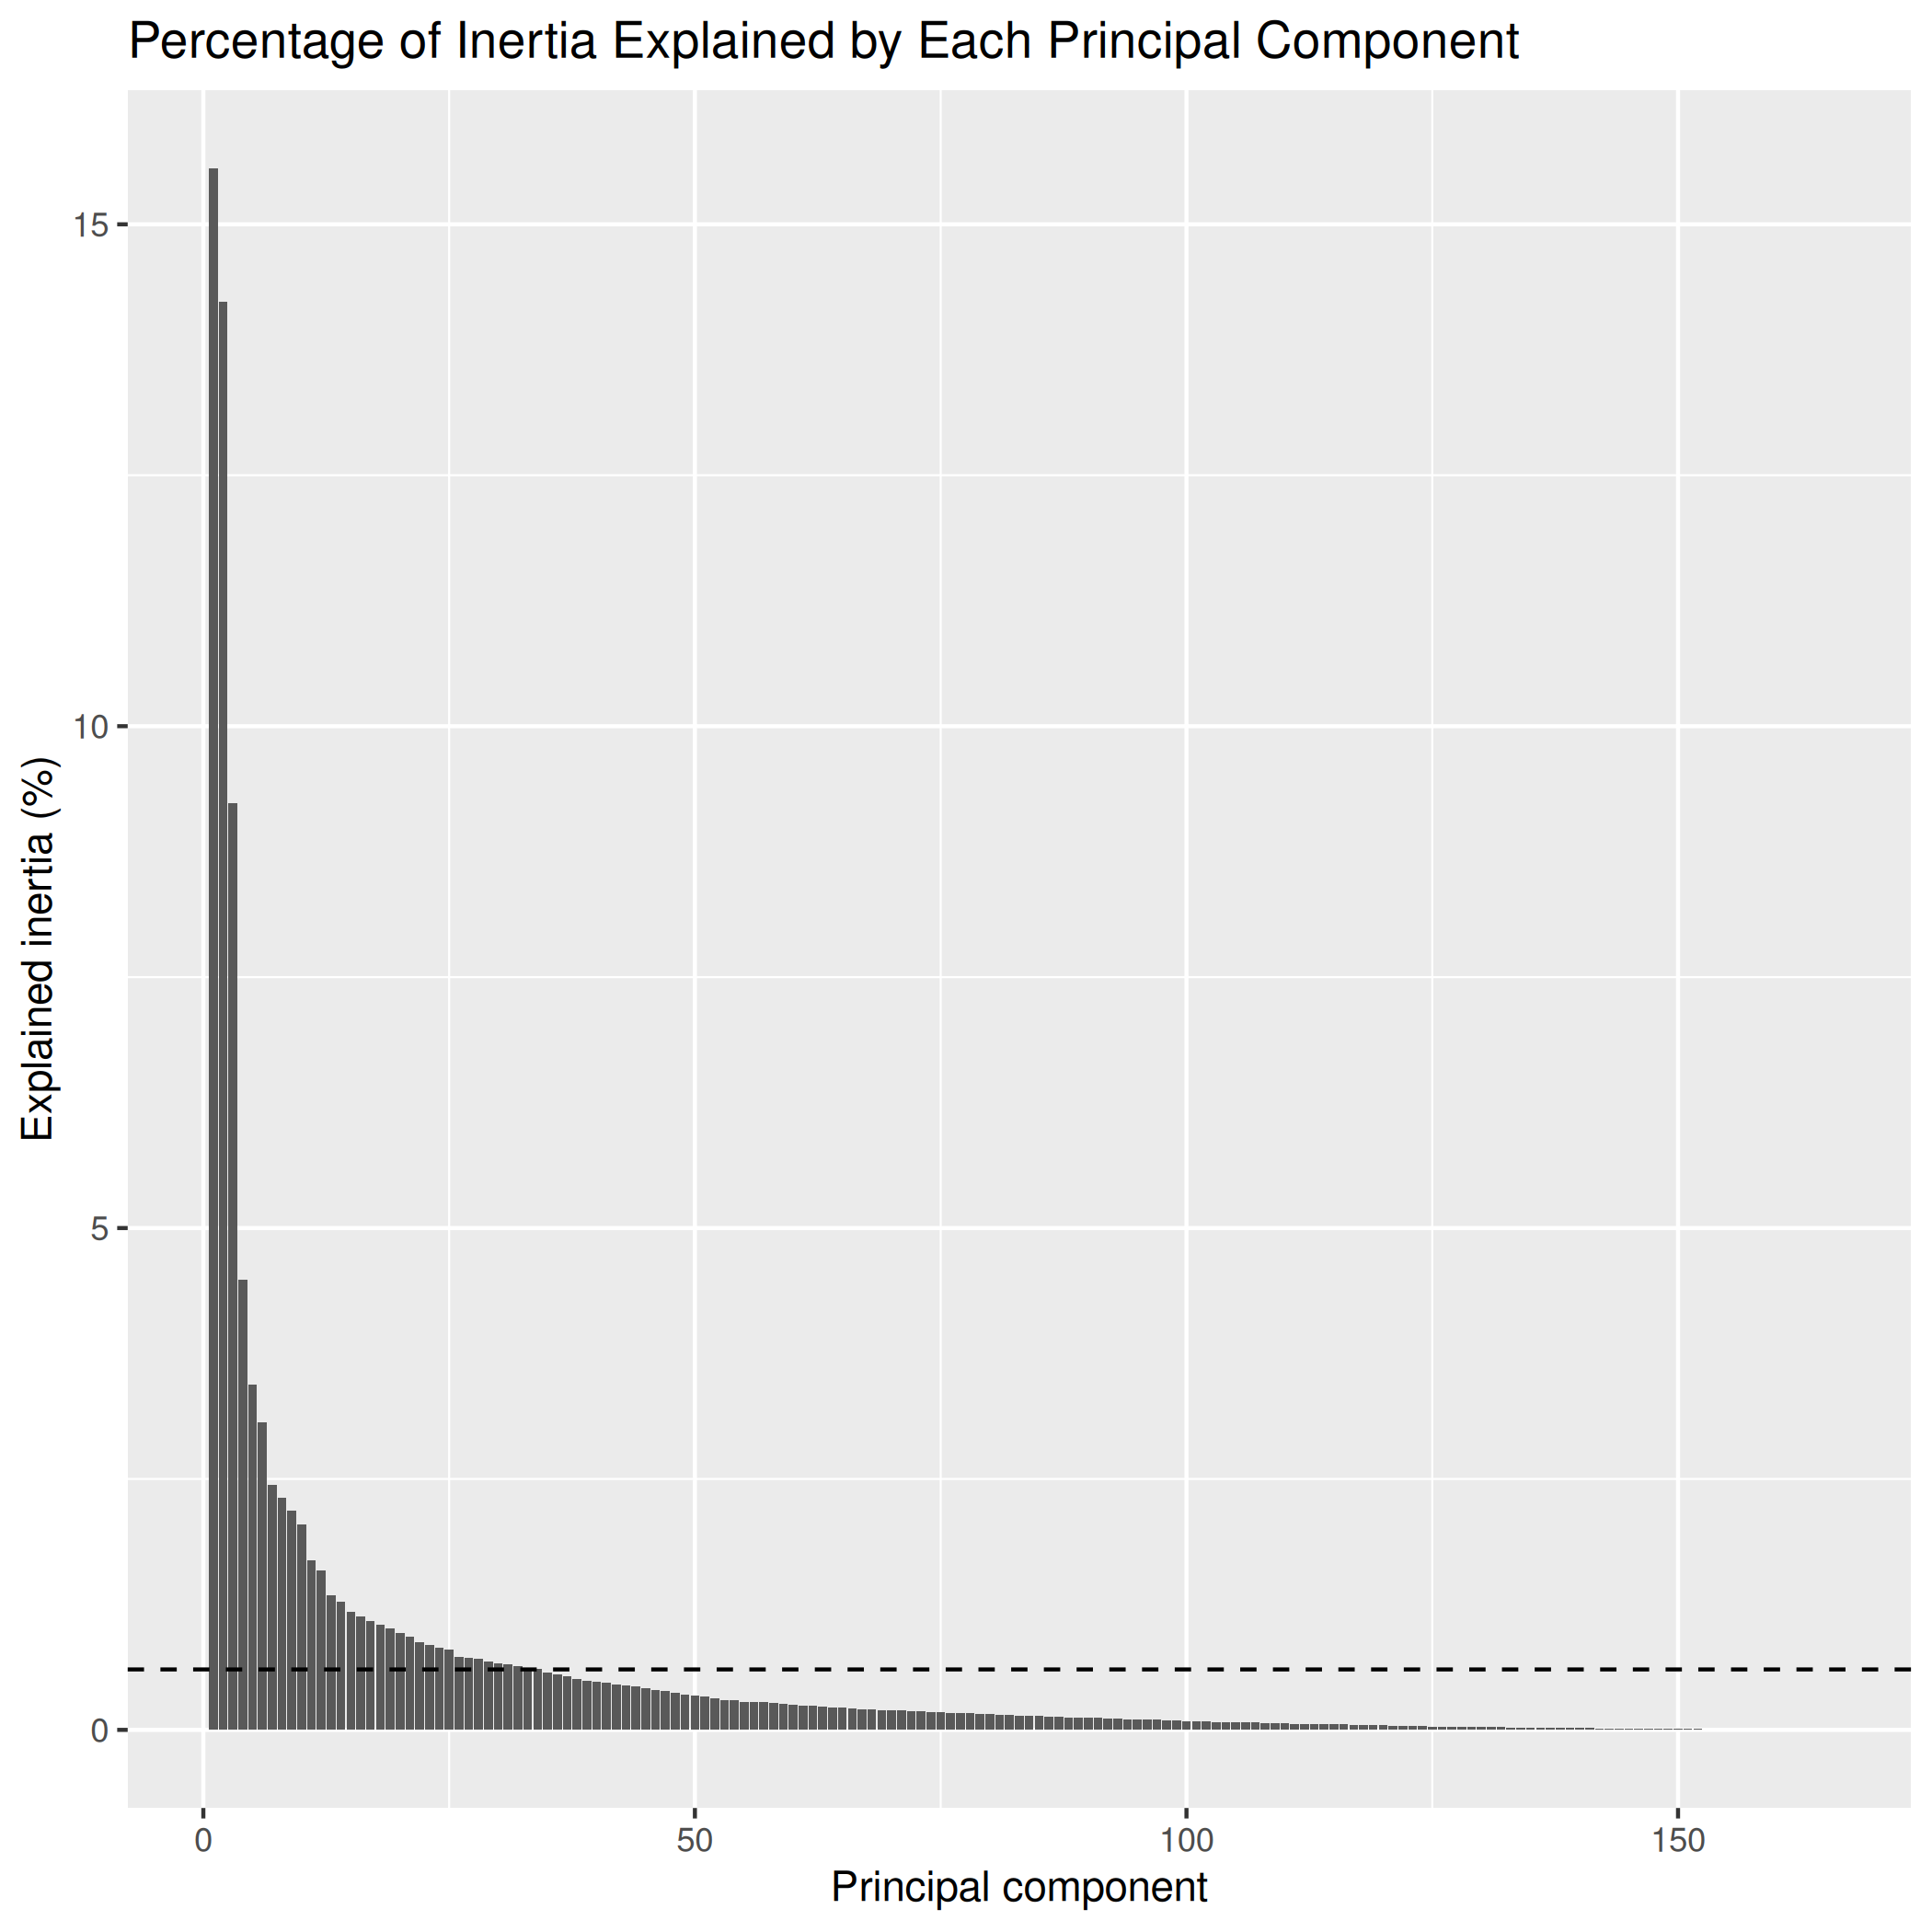
\includegraphics[width=0.92\columnwidth]{../output/part1/inertie_percentage.png}
\caption{Percentage of inertia explained by each principal component. The dashed horizontal line marks the average contribution \(100/165\).}
\label{fig:pca_inertia_percentage}
\end{figure}

\begin{table}[H]
\centering
\caption{Cumulative inertia and mean individual quality of representation for selected PCA subspaces.}
\label{tab:pca_subspace_summary}
\scriptsize
\begin{tabular}{ccc}
\toprule
Dimensions & Cumulative inertia (\%) & Mean individual \(\cos^2\) \\
\midrule
2  & 29.7942 & 0.2888 \\
4  & 43.5192 & 0.4283 \\
6  & 50.0195 & 0.4970 \\
10 & 59.0076 & 0.5900 \\
34 & 81.6010 & 0.8064 \\
\bottomrule
\end{tabular}
\end{table}

\begin{table}[H]
\centering
\caption{Ten variables with the largest contributions to PC1.}
\label{tab:pca_pc1_variables}
\scriptsize
\resizebox{\columnwidth}{!}{%
\begin{tabular}{lccccc}
\toprule
Variable & Contrib. & Corr. & \(\cos^2\) axis & \(\cos^2(1,2)\) & \(\cos^2(1{:}4)\) \\
\midrule
PAR\_ASE14 & 2.512 & -0.803 & 0.645 & 0.647 & 0.661 \\
PAR\_ASE15 & 2.335 & -0.774 & 0.600 & 0.600 & 0.604 \\
PAR\_ASE13 & 2.266 & -0.763 & 0.582 & 0.597 & 0.627 \\
PAR\_ASS   & 2.180 &  0.748 & 0.560 & 0.564 & 0.759 \\
PAR\_MFCC1 & 2.134 & -0.740 & 0.548 & 0.581 & 0.898 \\
PAR\_ASE17 & 2.083 & -0.731 & 0.535 & 0.552 & 0.577 \\
PAR\_SFM11 & 2.023 &  0.721 & 0.520 & 0.703 & 0.705 \\
PAR\_ASE18 & 2.020 & -0.720 & 0.519 & 0.532 & 0.562 \\
PAR\_ASE12 & 2.001 & -0.717 & 0.514 & 0.553 & 0.618 \\
PAR\_ASC\_V & 1.986 &  0.714 & 0.510 & 0.701 & 0.729 \\
\bottomrule
\end{tabular}}
\end{table}

\begin{table}[H]
\centering
\caption{Ten variables with the largest contributions to PC2.}
\label{tab:pca_pc2_variables}
\scriptsize
\resizebox{\columnwidth}{!}{%
\begin{tabular}{lccccc}
\toprule
Variable & Contrib. & Corr. & \(\cos^2\) axis & \(\cos^2(1,2)\) & \(\cos^2(1{:}4)\) \\
\midrule
PAR\_3RMS\_TCD & 1.659 &  0.624 & 0.390 & 0.424 & 0.469 \\
PAR\_ASE7 & 1.648 & -0.622 & 0.387 & 0.414 & 0.686 \\
PAR\_ASE8 & 1.641 & -0.621 & 0.385 & 0.385 & 0.580 \\
PAR\_ASEV22 & 1.617 &  0.616 & 0.380 & 0.392 & 0.493 \\
PAR\_3RMS\_TCD\_10FR\_MEAN & 1.569 &  0.607 & 0.369 & 0.405 & 0.448 \\
PAR\_ASEV26 & 1.564 &  0.606 & 0.367 & 0.372 & 0.493 \\
PAR\_ASEV27 & 1.515 &  0.596 & 0.356 & 0.373 & 0.450 \\
PAR\_ASEV24 & 1.500 &  0.594 & 0.352 & 0.354 & 0.475 \\
PAR\_ASEV25 & 1.488 &  0.591 & 0.349 & 0.351 & 0.480 \\
PAR\_ASEV23 & 1.468 &  0.587 & 0.345 & 0.349 & 0.470 \\
\bottomrule
\end{tabular}}
\end{table}

\begin{table}[H]
\centering
\caption{Ten variables with the largest contributions to PC3.}
\label{tab:pca_pc3_variables}
\scriptsize
\resizebox{\columnwidth}{!}{%
\begin{tabular}{lccccc}
\toprule
Variable & Contrib. & Corr. & \(\cos^2\) axis & \(\cos^2(1,2)\) & \(\cos^2(1{:}4)\) \\
\midrule
PAR\_ASE23 & 3.612 & -0.742 & 0.551 & 0.085 & 0.670 \\
PAR\_ASE25 & 3.570 & -0.738 & 0.544 & 0.165 & 0.747 \\
PAR\_ASE24 & 3.364 & -0.716 & 0.513 & 0.122 & 0.677 \\
PAR\_ASE22 & 3.223 & -0.701 & 0.491 & 0.138 & 0.650 \\
PAR\_1RMS\_TCD & 3.067 & -0.684 & 0.467 & 0.294 & 0.762 \\
PAR\_ASE26 & 2.966 & -0.672 & 0.452 & 0.240 & 0.711 \\
PAR\_ASE27 & 2.582 & -0.627 & 0.393 & 0.284 & 0.681 \\
PAR\_2RMS\_TCD & 2.516 & -0.619 & 0.383 & 0.384 & 0.768 \\
PAR\_ASC & 2.466 & -0.613 & 0.376 & 0.373 & 0.778 \\
PAR\_2RMS\_TCD\_10FR\_MEAN & 2.431 & -0.609 & 0.370 & 0.364 & 0.735 \\
\bottomrule
\end{tabular}}
\end{table}

\begin{table}[H]
\centering
\caption{Ten variables with the largest contributions to PC4.}
\label{tab:pca_pc4_variables}
\scriptsize
\resizebox{\columnwidth}{!}{%
\begin{tabular}{lccccc}
\toprule
Variable & Contrib. & Corr. & \(\cos^2\) axis & \(\cos^2(1,2)\) & \(\cos^2(1{:}4)\) \\
\midrule
PAR\_ASE34 & 3.761 & -0.528 & 0.278 & 0.017 & 0.573 \\
PAR\_SFMV22 & 3.472 &  0.507 & 0.257 & 0.156 & 0.426 \\
PAR\_ASE5 & 3.367 &  0.499 & 0.249 & 0.411 & 0.757 \\
PAR\_ASE6 & 3.363 &  0.499 & 0.249 & 0.419 & 0.746 \\
PAR\_ASE4 & 2.812 &  0.456 & 0.208 & 0.402 & 0.722 \\
PAR\_ASE33 & 2.808 & -0.456 & 0.208 & 0.083 & 0.459 \\
PAR\_SFM22 & 2.688 & -0.446 & 0.199 & 0.088 & 0.425 \\
PAR\_ASE7 & 2.662 &  0.444 & 0.197 & 0.414 & 0.686 \\
PAR\_SFMV21 & 2.654 &  0.443 & 0.197 & 0.305 & 0.501 \\
PAR\_ASE3 & 2.113 &  0.396 & 0.157 & 0.387 & 0.665 \\
\bottomrule
\end{tabular}}
\end{table}

\begin{table}[H]
\centering
\caption{Variables best represented on the first principal plane.}
\label{tab:pca_best_plane12}
\scriptsize
\begin{tabular}{lc}
\toprule
Variable & \(\cos^2(1,2)\) \\
\midrule
PAR\_SC\_V & 0.780 \\
PAR\_SFM15 & 0.719 \\
PAR\_SFM11 & 0.703 \\
PAR\_SFM12 & 0.703 \\
PAR\_ASC\_V & 0.701 \\
PAR\_SFM14 & 0.691 \\
PAR\_SFM16 & 0.676 \\
PAR\_SFM10 & 0.674 \\
PAR\_SFM13 & 0.663 \\
PAR\_ASE14 & 0.647 \\
PAR\_SFM9 & 0.635 \\
PAR\_ASE15 & 0.600 \\
PAR\_ASE13 & 0.597 \\
PAR\_SFM17 & 0.596 \\
PAR\_MFCC1 & 0.581 \\
\bottomrule
\end{tabular}
\end{table}

\begin{table}[H]
\centering
\caption{Variables best represented on the first four principal components.}
\label{tab:pca_best_first4}
\scriptsize
\begin{tabular}{lc}
\toprule
Variable & \(\cos^2(1{:}4)\) \\
\midrule
PAR\_MFCC1 & 0.898 \\
PAR\_ZCD & 0.841 \\
PAR\_SC\_V & 0.815 \\
PAR\_SC & 0.799 \\
PAR\_ASC & 0.778 \\
PAR\_2RMS\_TCD & 0.768 \\
PAR\_1RMS\_TCD & 0.762 \\
PAR\_ASS & 0.759 \\
PAR\_ASE5 & 0.757 \\
PAR\_SFM15 & 0.752 \\
PAR\_ASE25 & 0.747 \\
PAR\_ASE6 & 0.746 \\
PAR\_SFM16 & 0.746 \\
PAR\_2RMS\_TCD\_10FR\_MEAN & 0.735 \\
PAR\_ASC\_V & 0.729 \\
\bottomrule
\end{tabular}
\end{table}

\begin{table}[H]
\centering
\caption{Counts of well-represented variables in the PCA variable space.}
\label{tab:pca_representation_counts}
\scriptsize
\begin{tabular}{lc}
\toprule
Criterion & Count \\
\midrule
Variables with \(\cos^2(1,2)\geq 0.5\) & 24 \\
Variables with \(\cos^2(1,2)\geq 0.7\) & 5 \\
Variables with \(\cos^2(1{:}4)\geq 0.5\) & 69 \\
Variables with \(\cos^2(1{:}4)\geq 0.7\) & 20 \\
\bottomrule
\end{tabular}
\end{table}

\subsection{Silhouette Criterion}
\label{subsec:silhouette}
For the clustering step, the number of clusters is selected by maximizing the average silhouette width. For an observation \(x_i\), the silhouette index compares the average dissimilarity to its own cluster with the smallest average dissimilarity to another cluster \cite{rousseeuw1987}:
\begin{equation}
\mathrm{sil}(x_i)=\frac{b_i-a_i}{\max(a_i,b_i)}.
\label{eq:silhouette}
\end{equation}
Here, \(a_i\) is the average distance from \(x_i\) to the observations of its own cluster, whereas \(b_i\) is the smallest average distance from \(x_i\) to another cluster. Larger values indicate that the observation is better assigned to its cluster and more clearly separated from the others.

\subsection{Silhouette Plots}
\label{subsec:silhouette_plots}
The following figures display the silhouette plots obtained for Ward clustering and for the true genre partition, for each retained PCA dimension and for both preprocessing modes.

\begin{figure}[H]
\centering
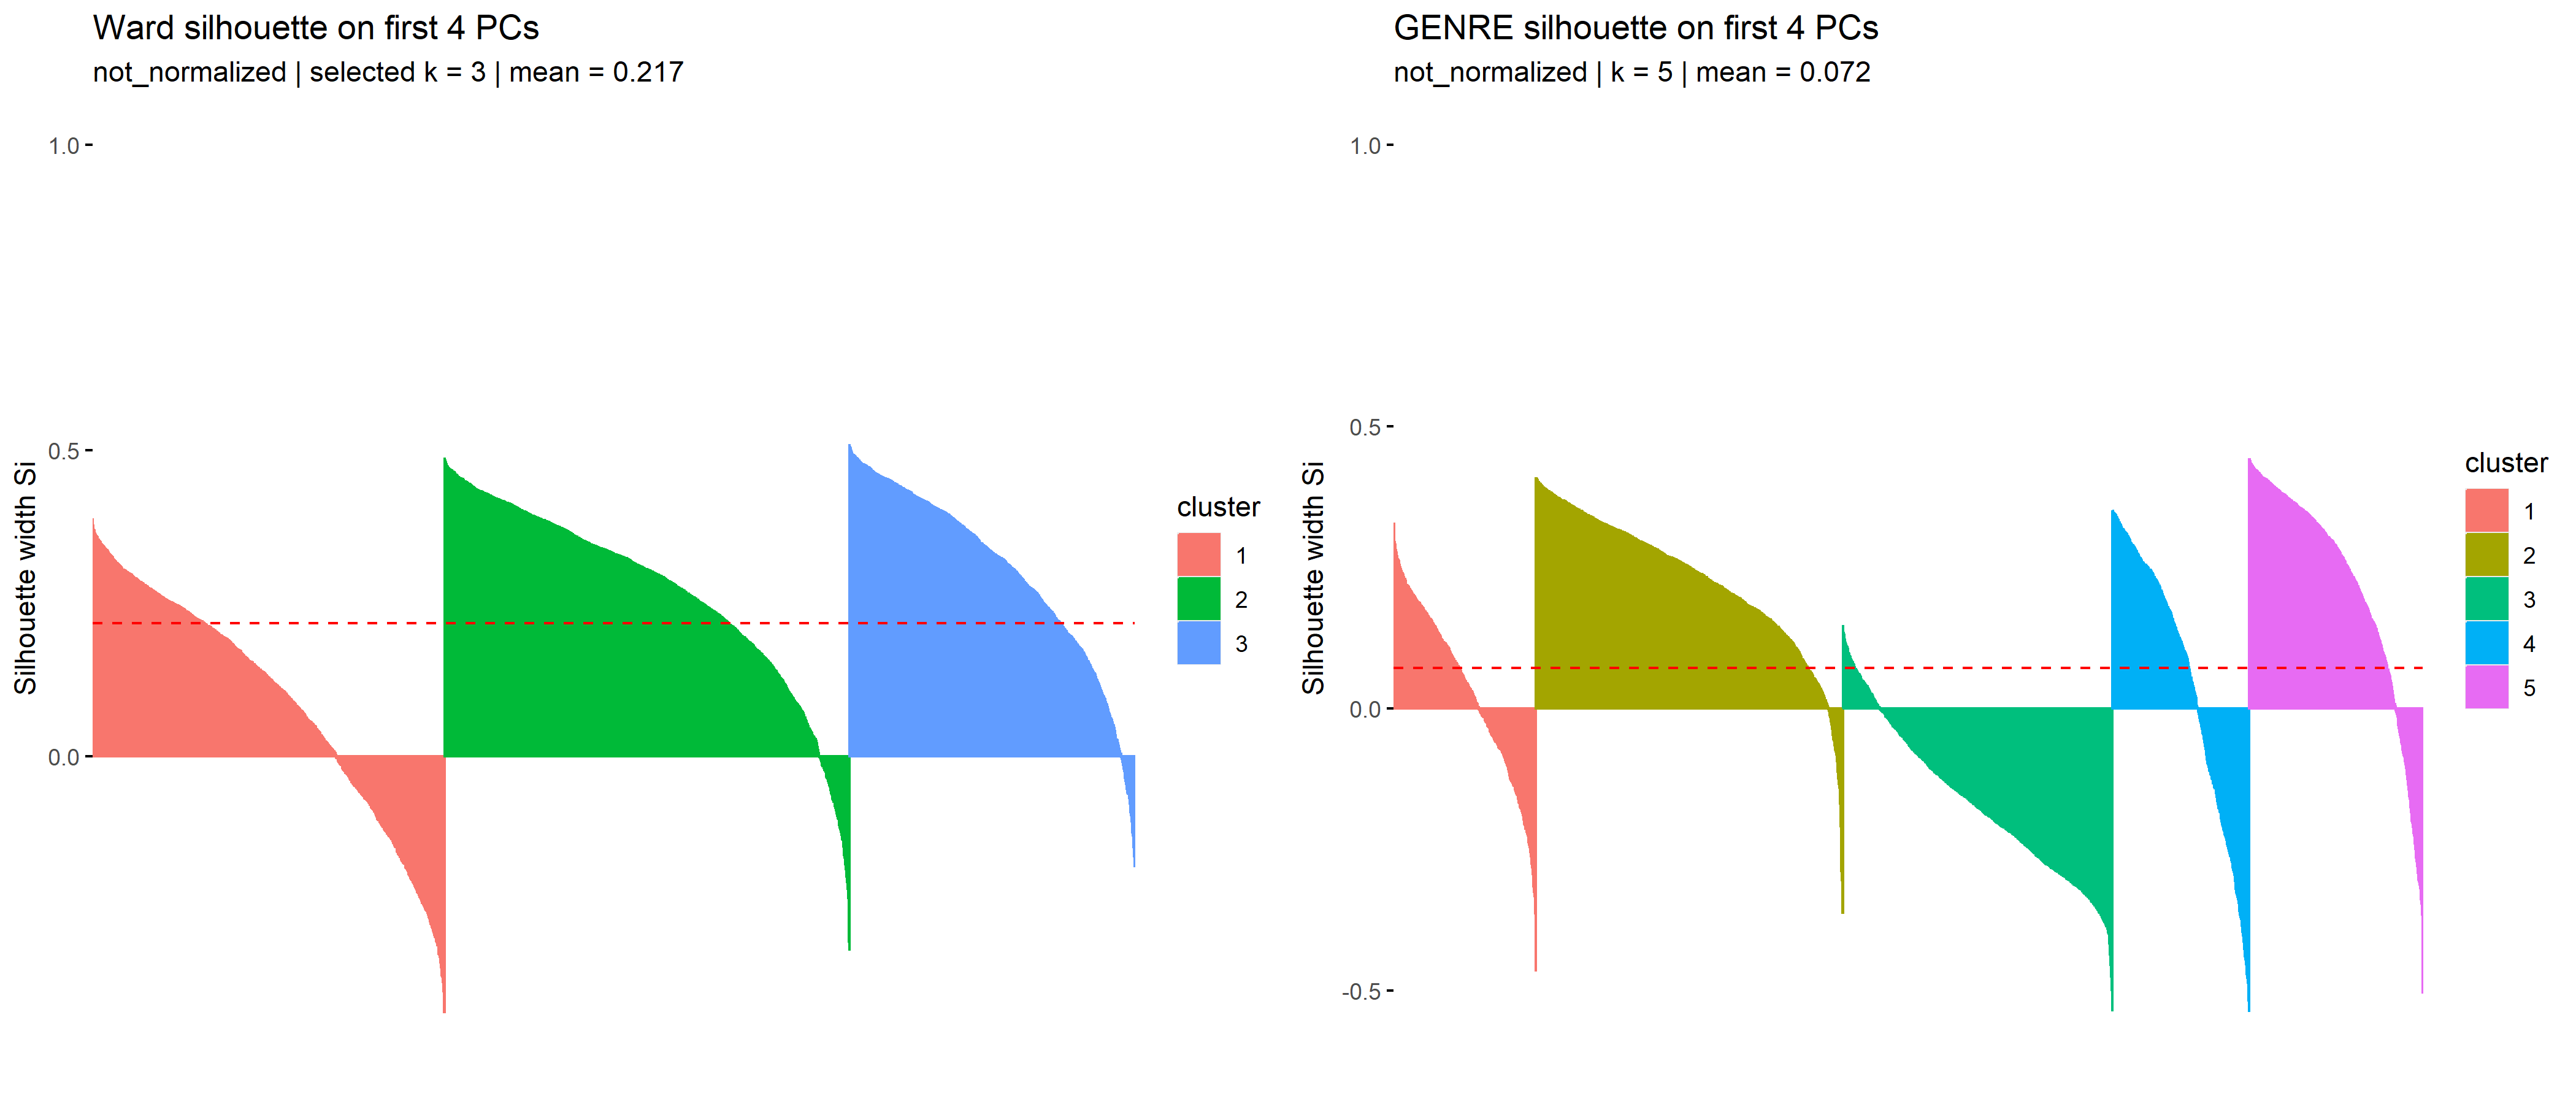
\includegraphics[width=\columnwidth]{../output/part1/hclust_pca/not_normalized/silhouette_pca_04_components.png}
\caption{Silhouette plots for the non-normalized PCA scores with \(d=4\) retained components.}
\label{fig:silhouette_not_normalized_4}
\end{figure}

\begin{figure}[H]
\centering
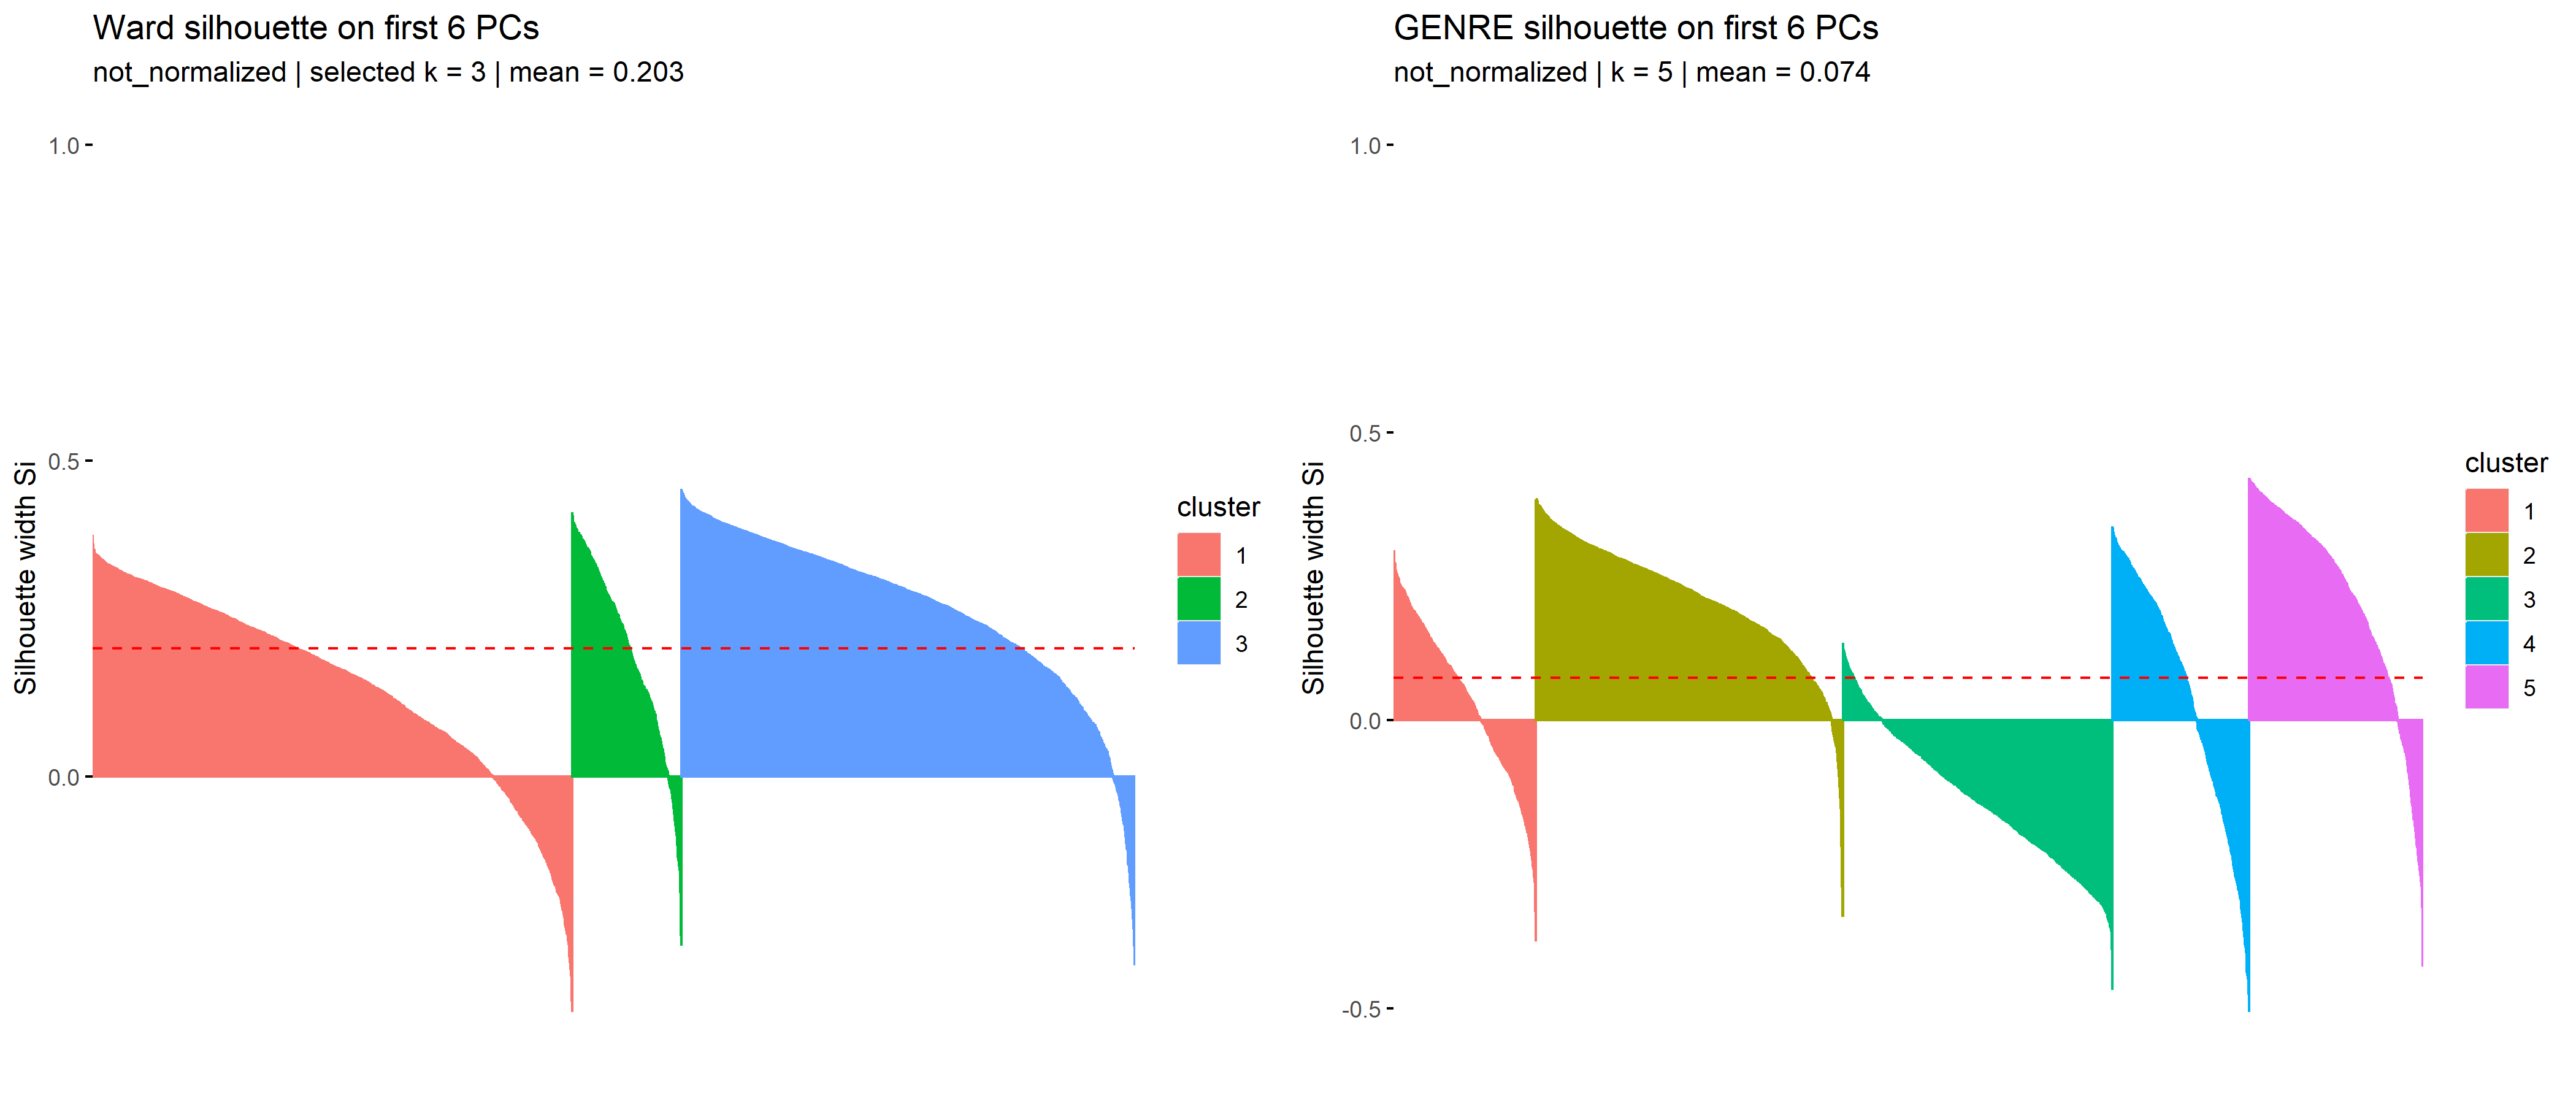
\includegraphics[width=\columnwidth]{../output/part1/hclust_pca/not_normalized/silhouette_pca_06_components.png}
\caption{Silhouette plots for the non-normalized PCA scores with \(d=6\) retained components.}
\label{fig:silhouette_not_normalized_6}
\end{figure}

\begin{figure}[H]
\centering
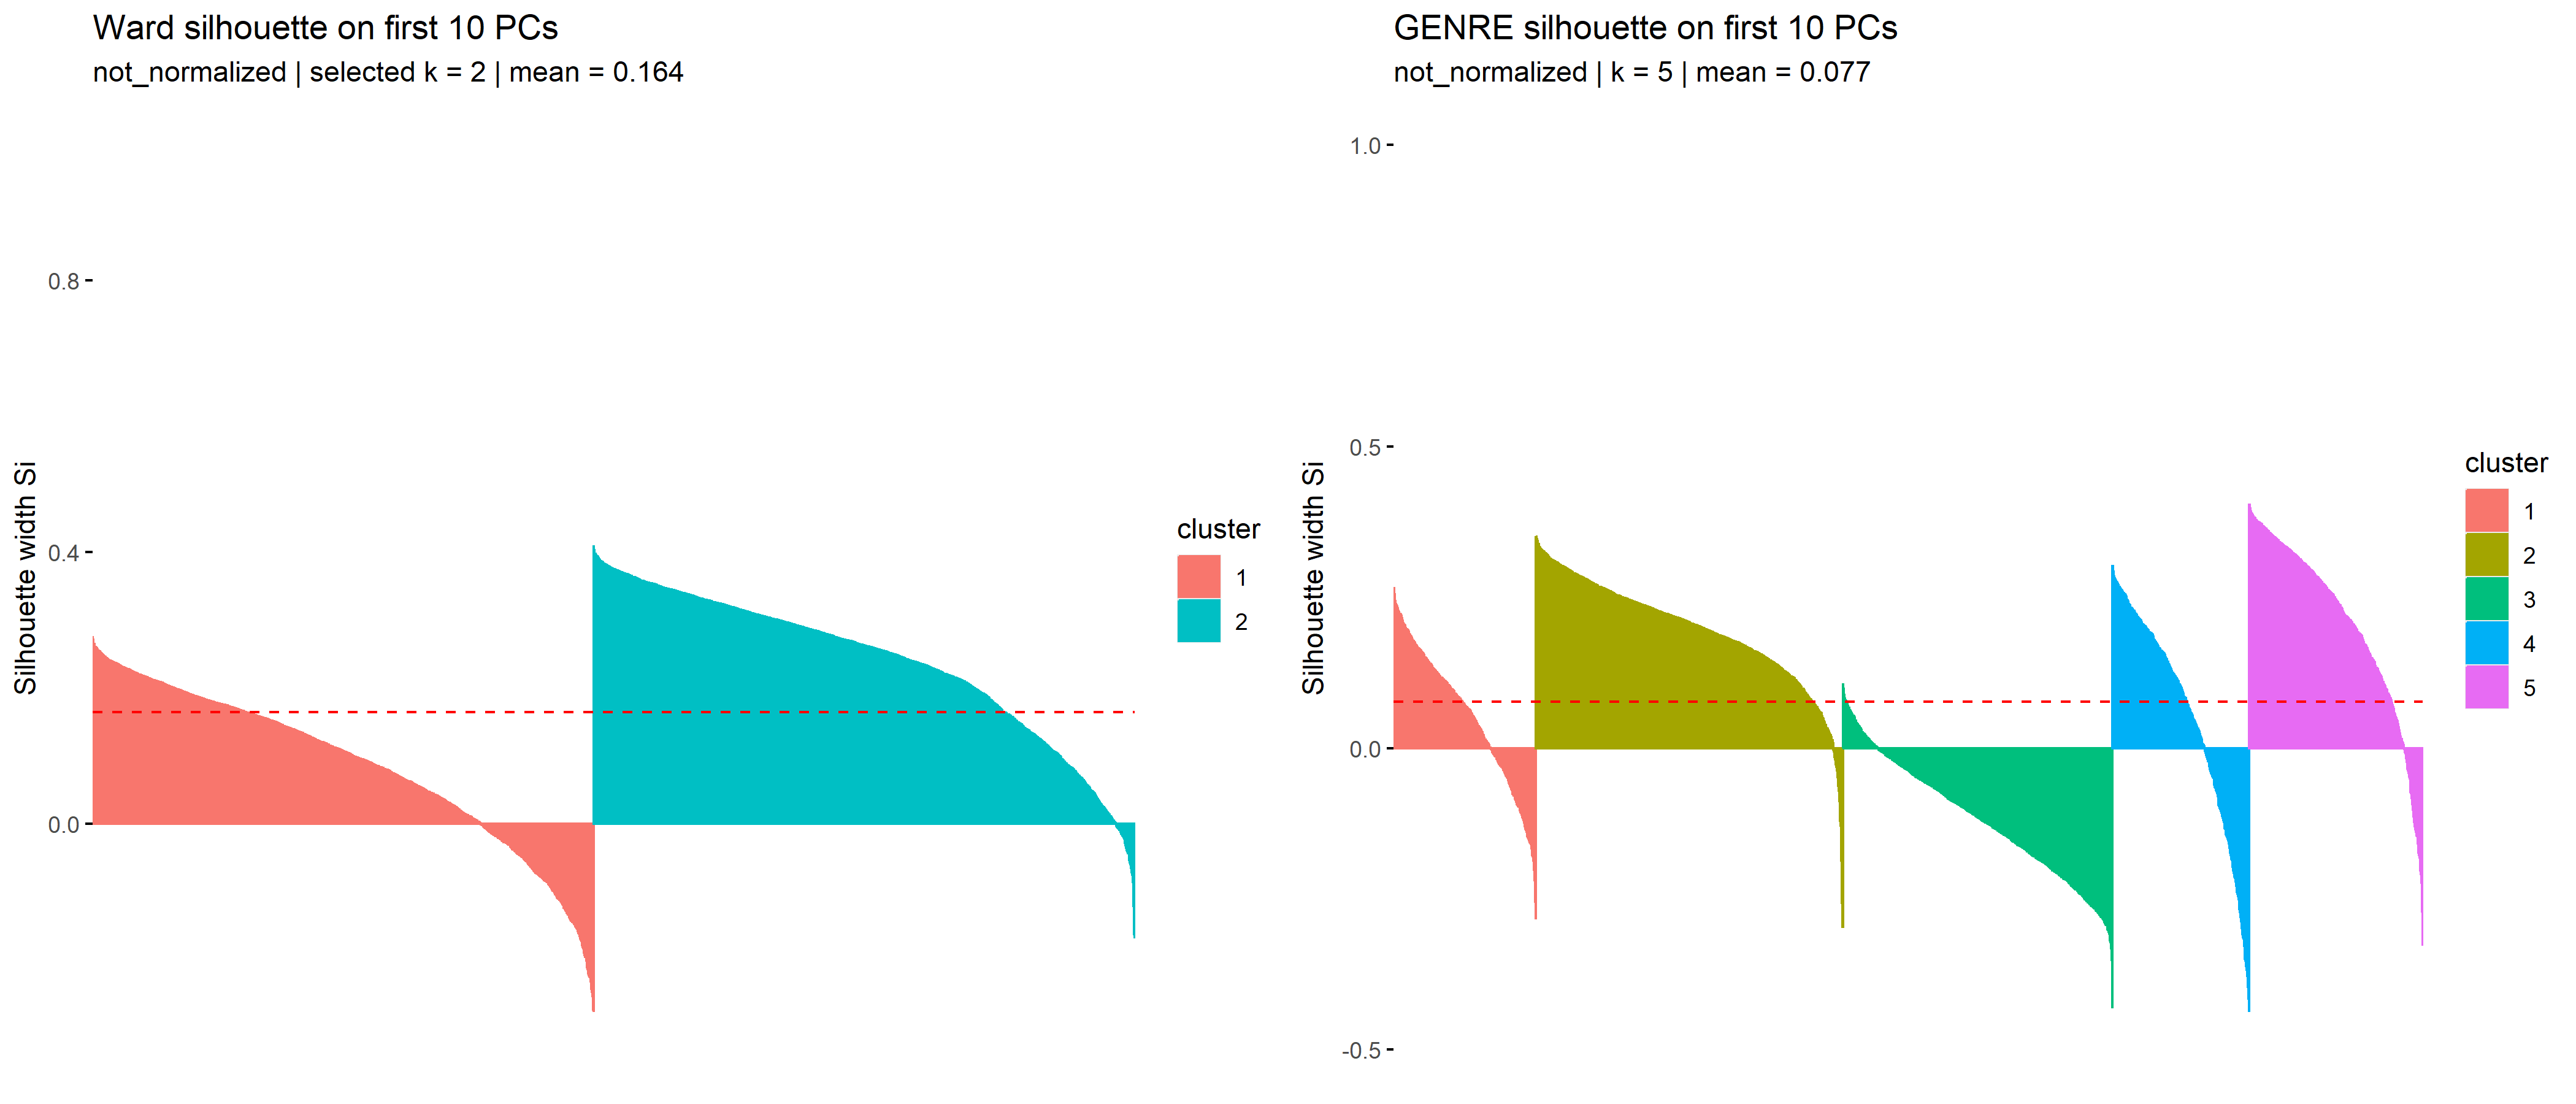
\includegraphics[width=\columnwidth]{../output/part1/hclust_pca/not_normalized/silhouette_pca_10_components.png}
\caption{Silhouette plots for the non-normalized PCA scores with \(d=10\) retained components.}
\label{fig:silhouette_not_normalized_10}
\end{figure}

\begin{figure}[H]
\centering
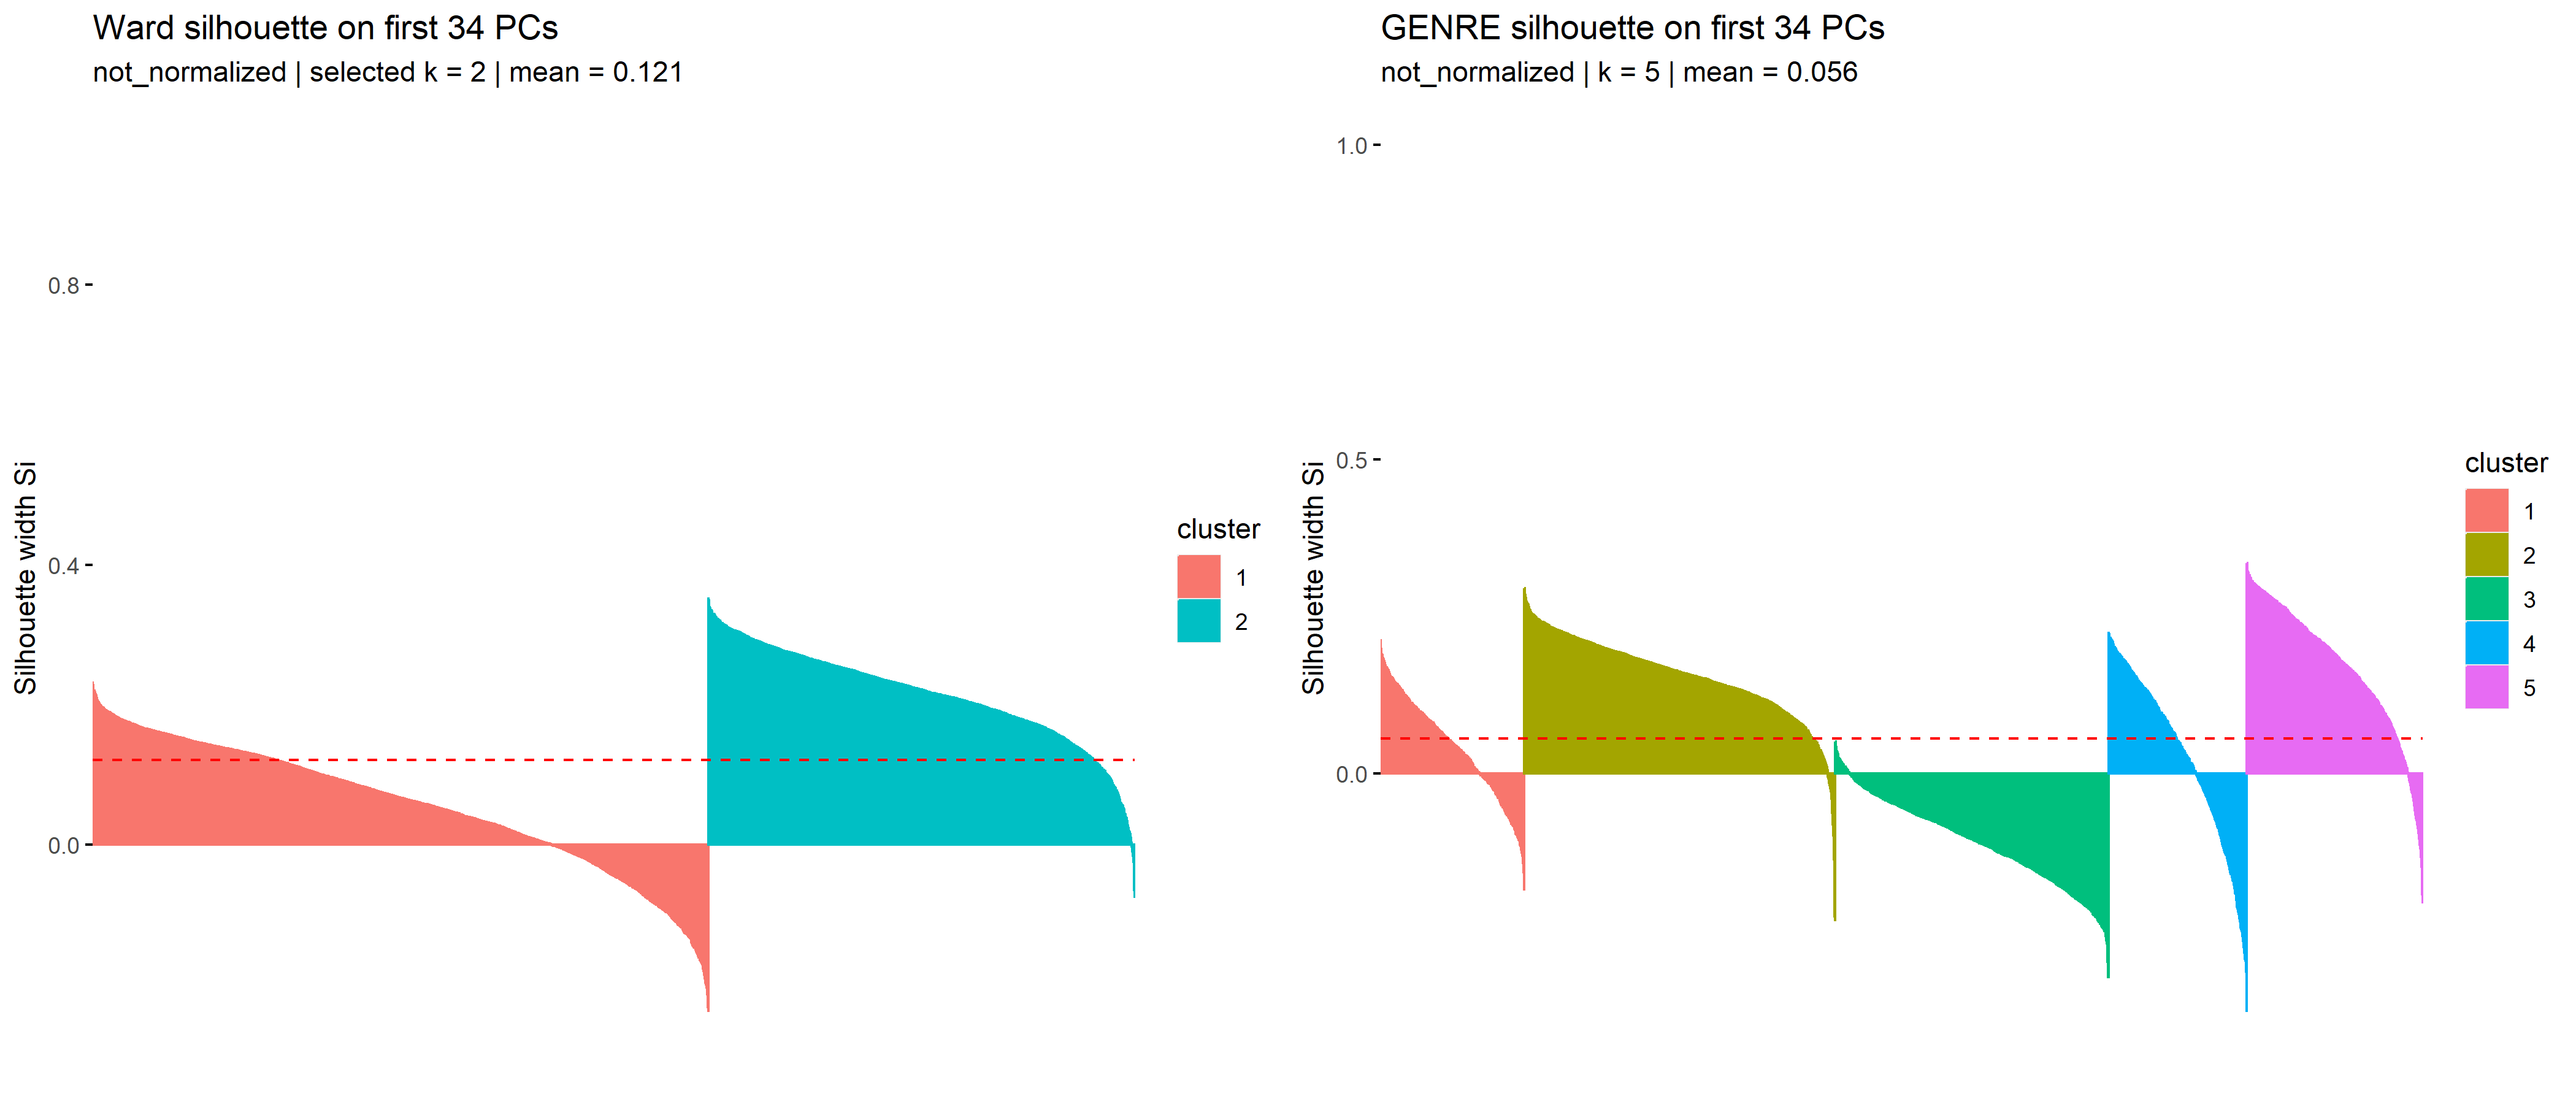
\includegraphics[width=\columnwidth]{../output/part1/hclust_pca/not_normalized/silhouette_pca_34_components.png}
\caption{Silhouette plots for the non-normalized PCA scores with \(d=34\) retained components.}
\label{fig:silhouette_not_normalized_34}
\end{figure}

\begin{figure}[H]
\centering
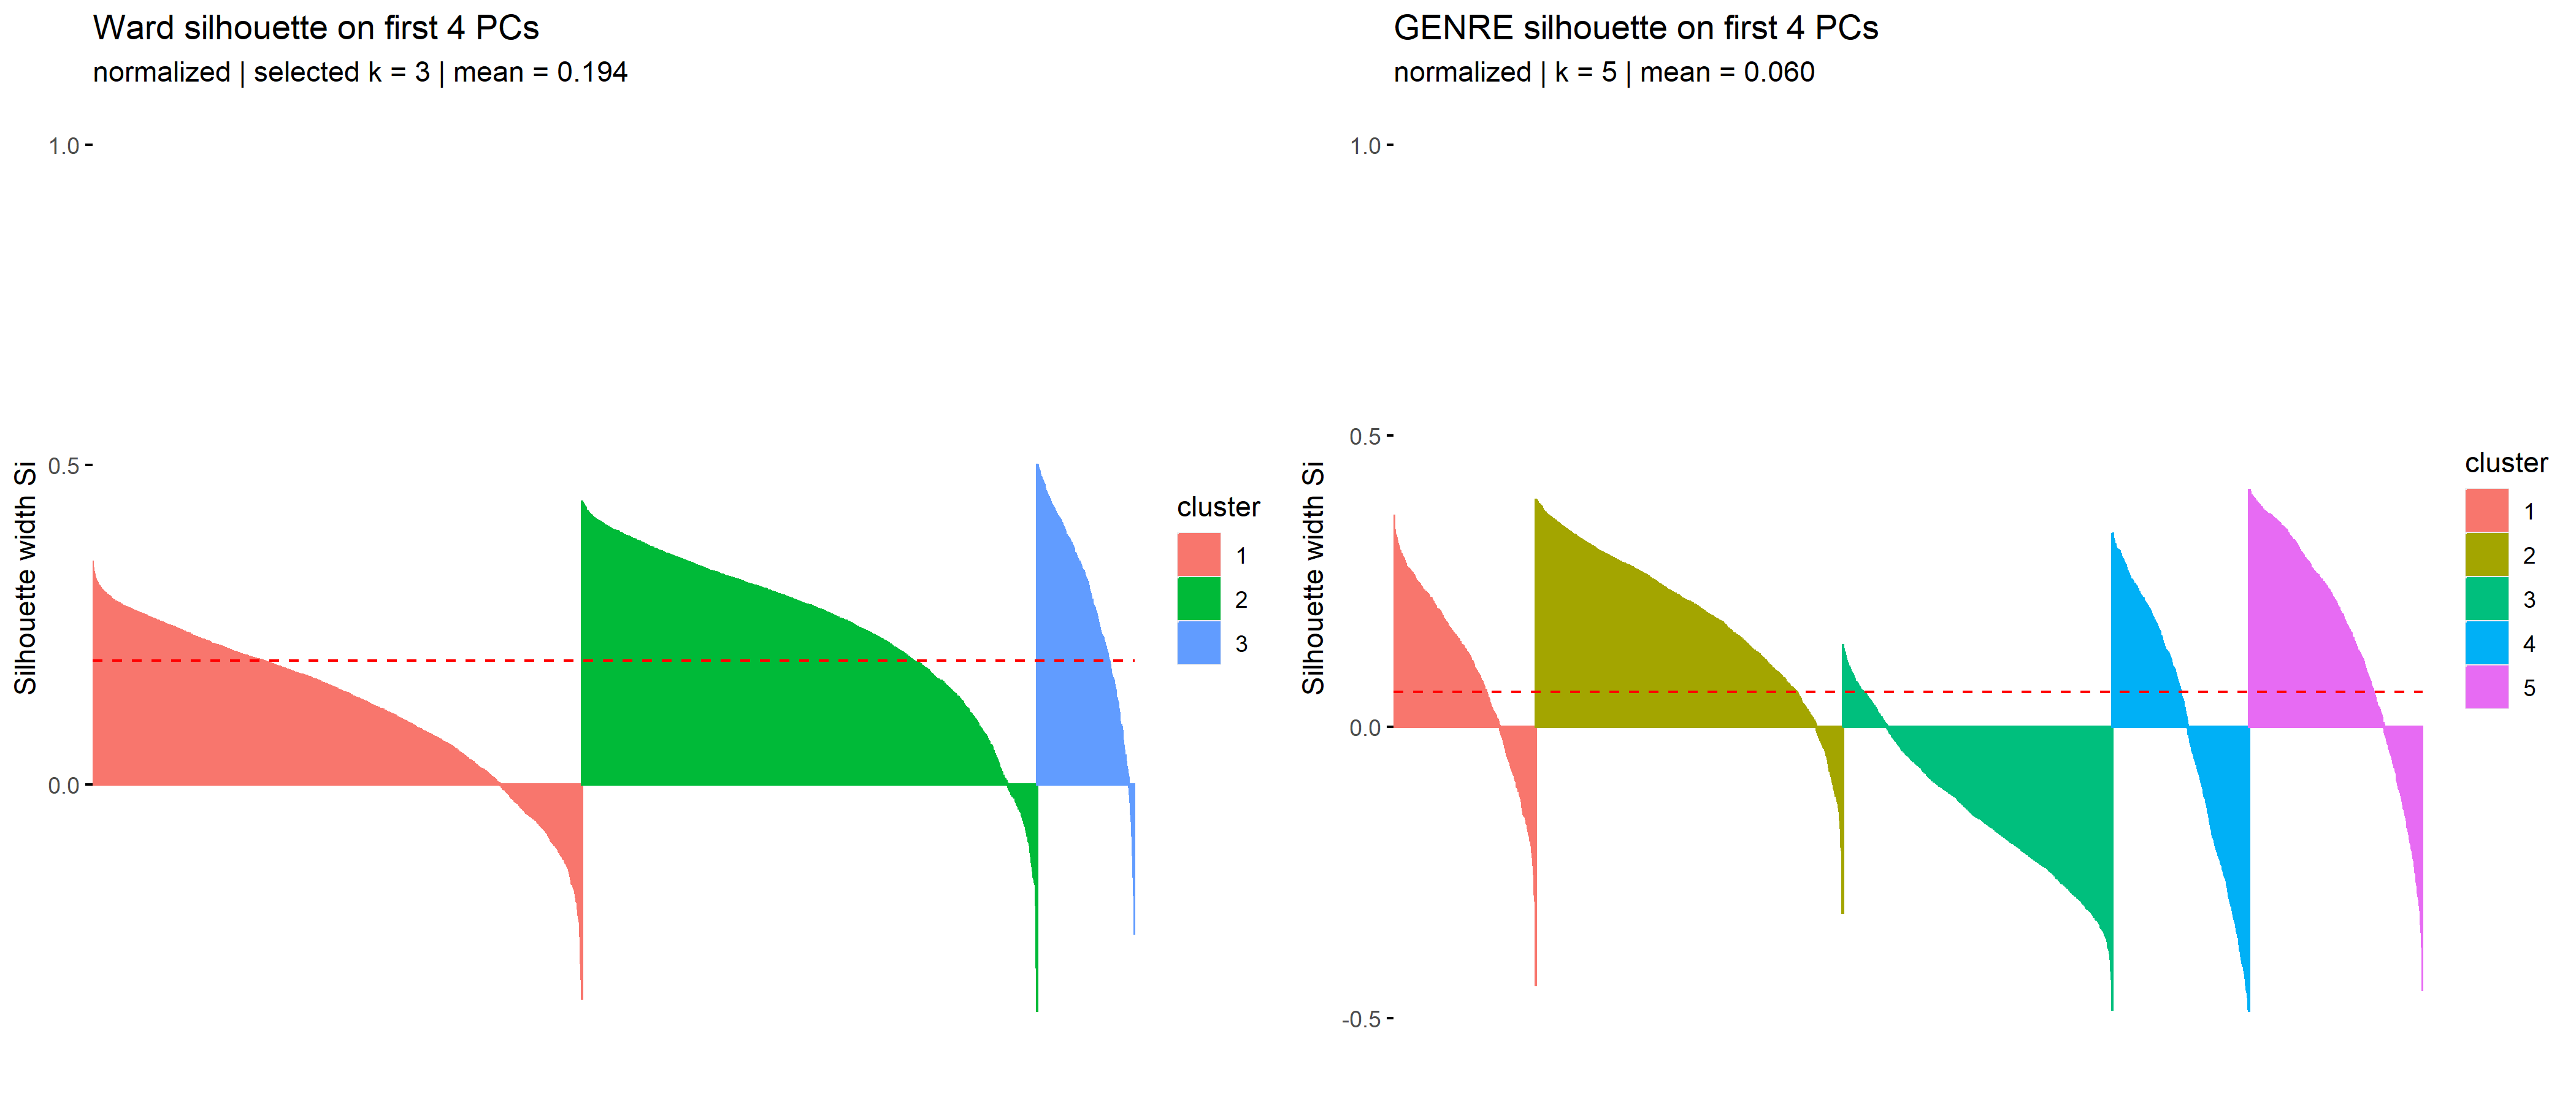
\includegraphics[width=\columnwidth]{../output/part1/hclust_pca/normalized/silhouette_pca_04_components.png}
\caption{Silhouette plots for the normalized PCA scores with \(d=4\) retained components.}
\label{fig:silhouette_normalized_4}
\end{figure}

\begin{figure}[H]
\centering
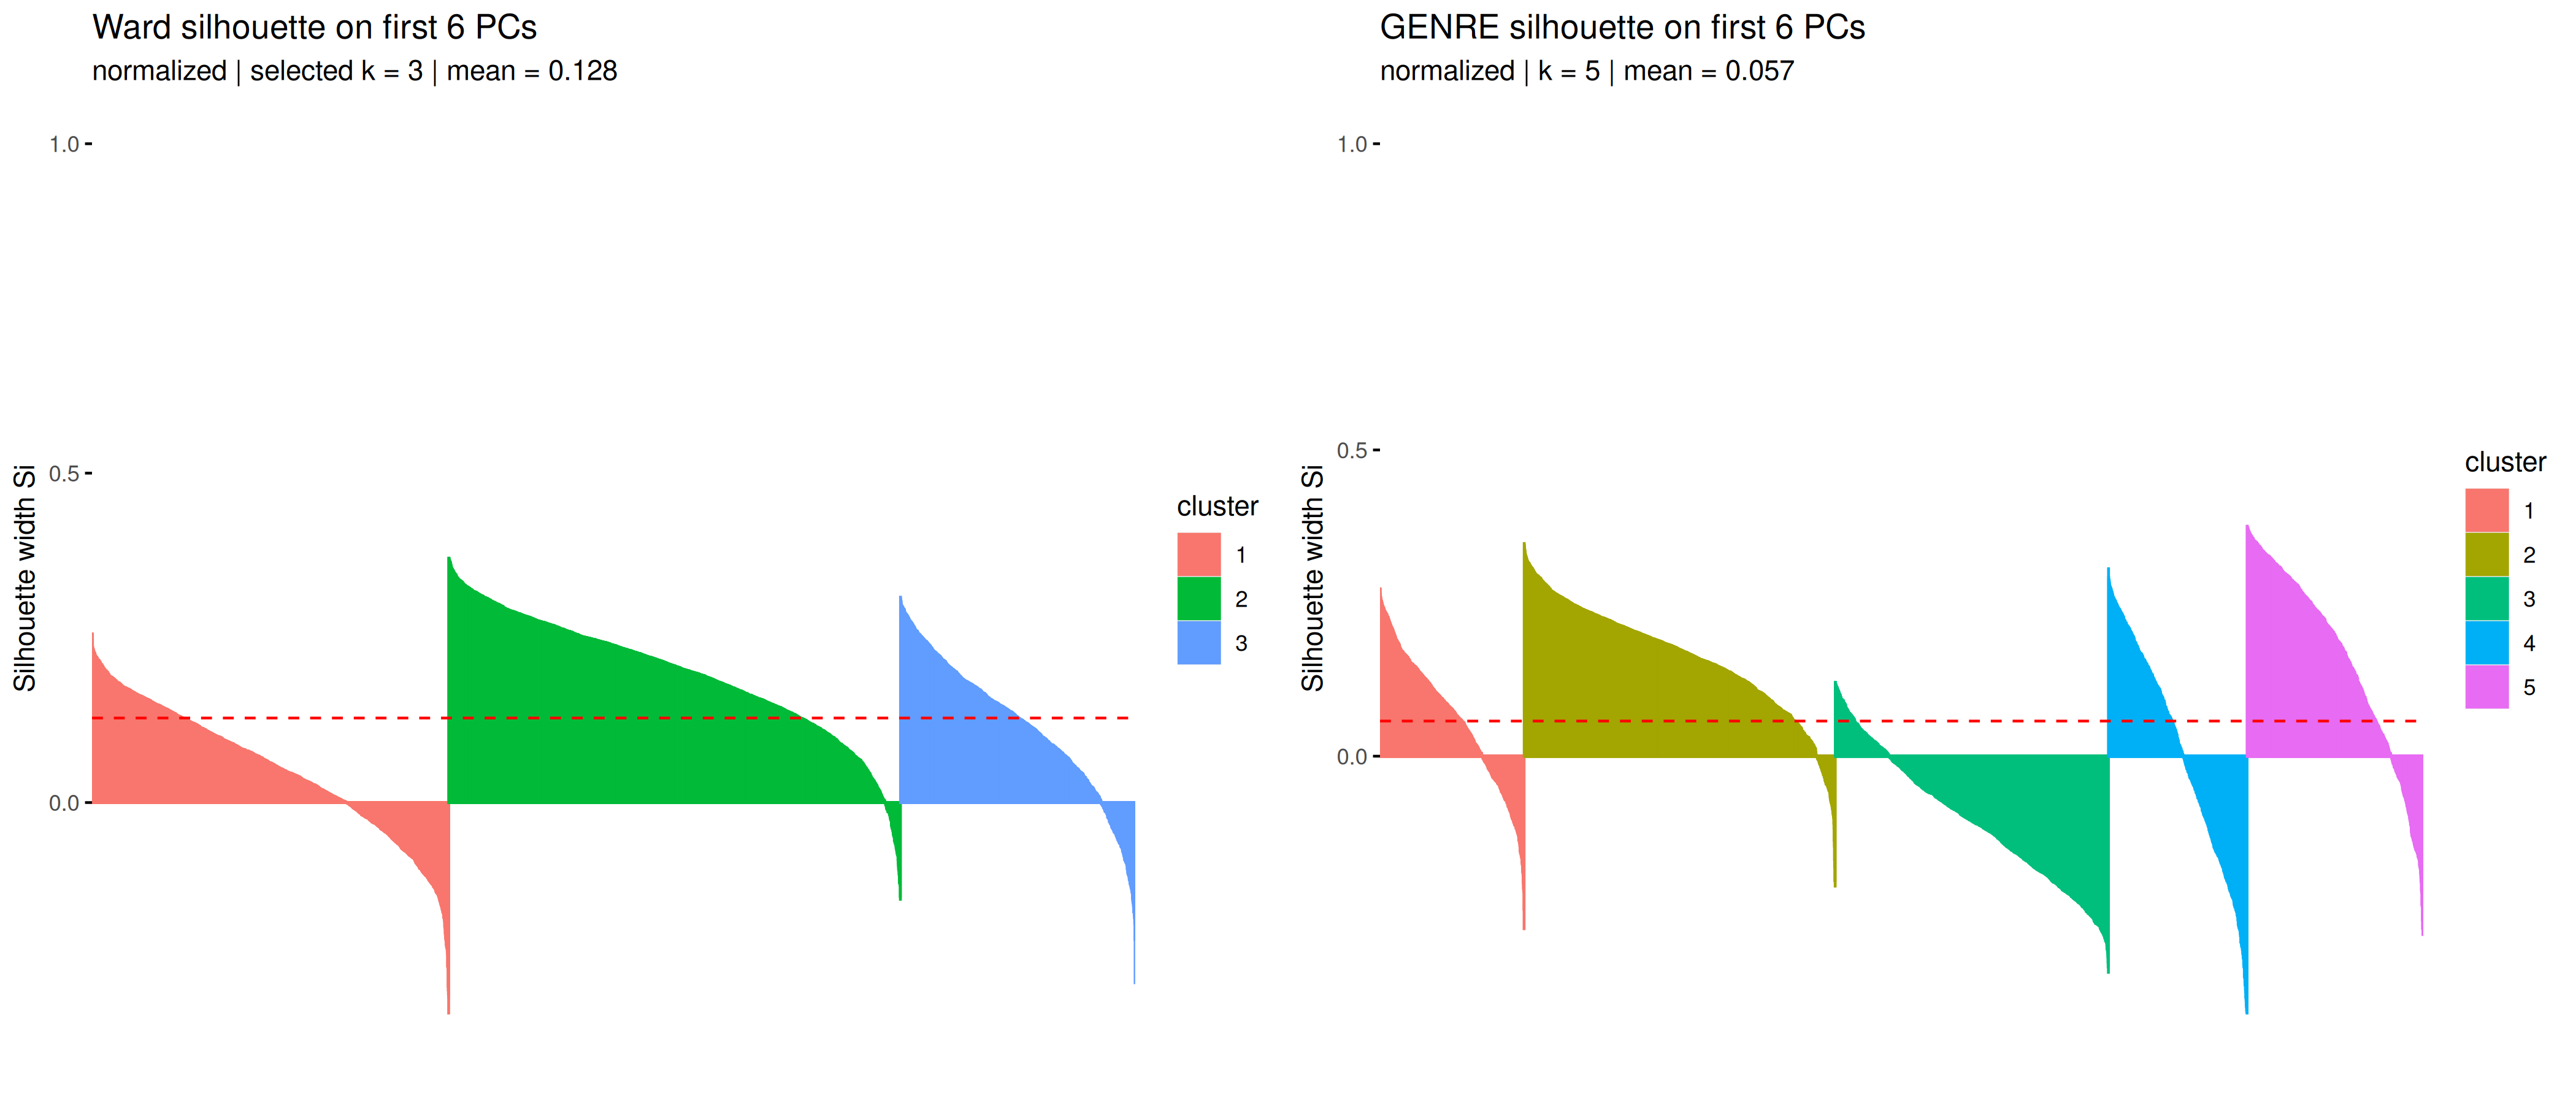
\includegraphics[width=\columnwidth]{../output/part1/hclust_pca/normalized/silhouette_pca_06_components.png}
\caption{Silhouette plots for the normalized PCA scores with \(d=6\) retained components.}
\label{fig:silhouette_normalized_6}
\end{figure}

\begin{figure}[H]
\centering
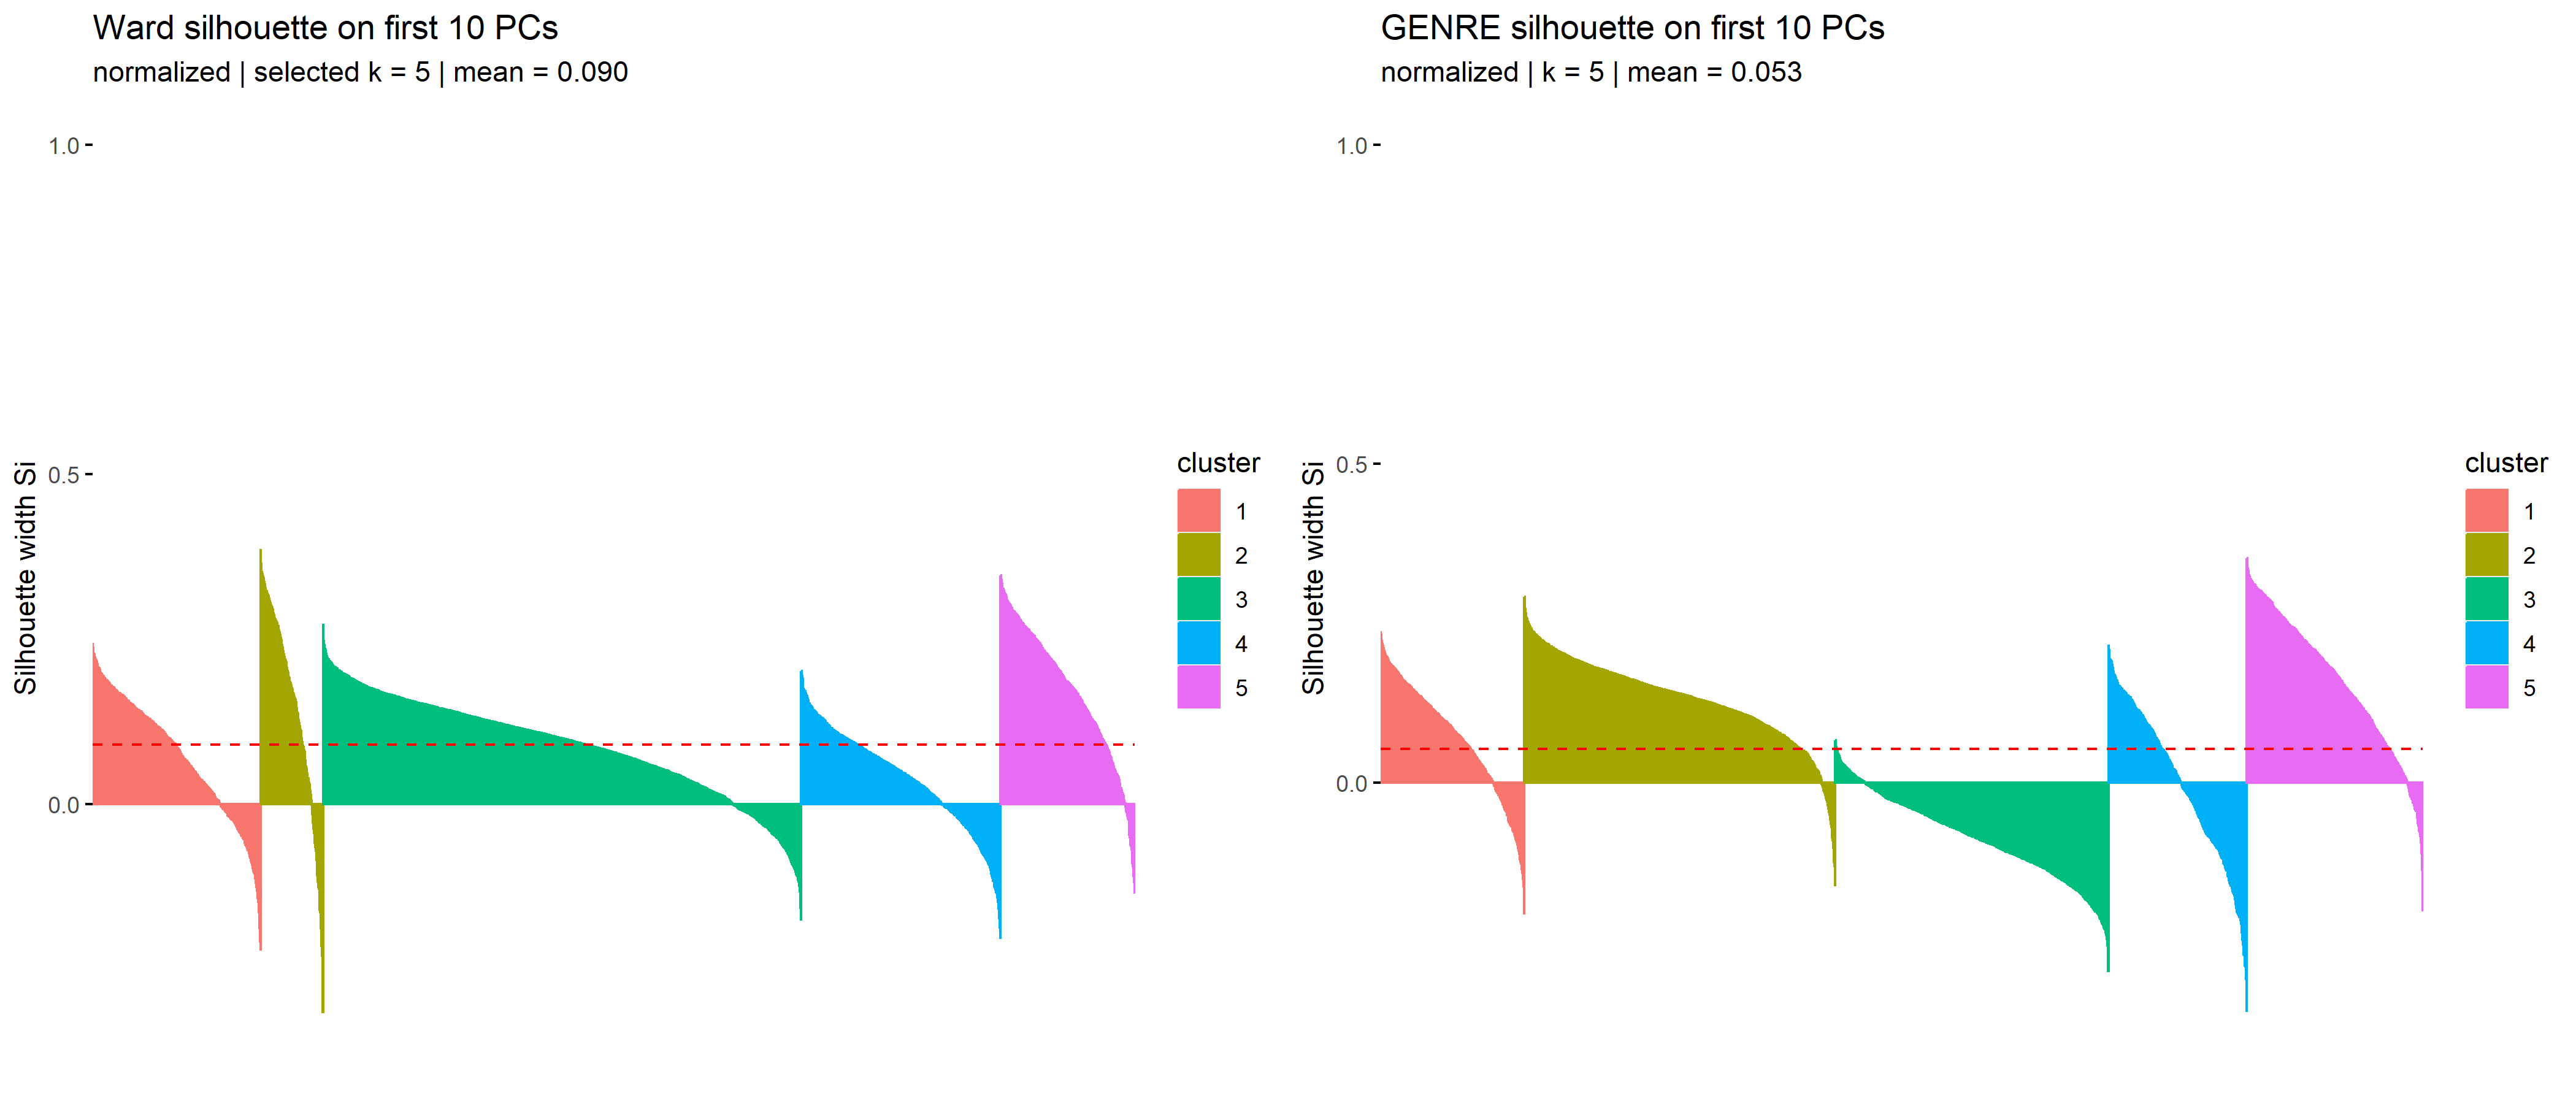
\includegraphics[width=\columnwidth]{../output/part1/hclust_pca/normalized/silhouette_pca_10_components.png}
\caption{Silhouette plots for the normalized PCA scores with \(d=10\) retained components.}
\label{fig:silhouette_normalized_10}
\end{figure}

\begin{figure}[H]
\centering
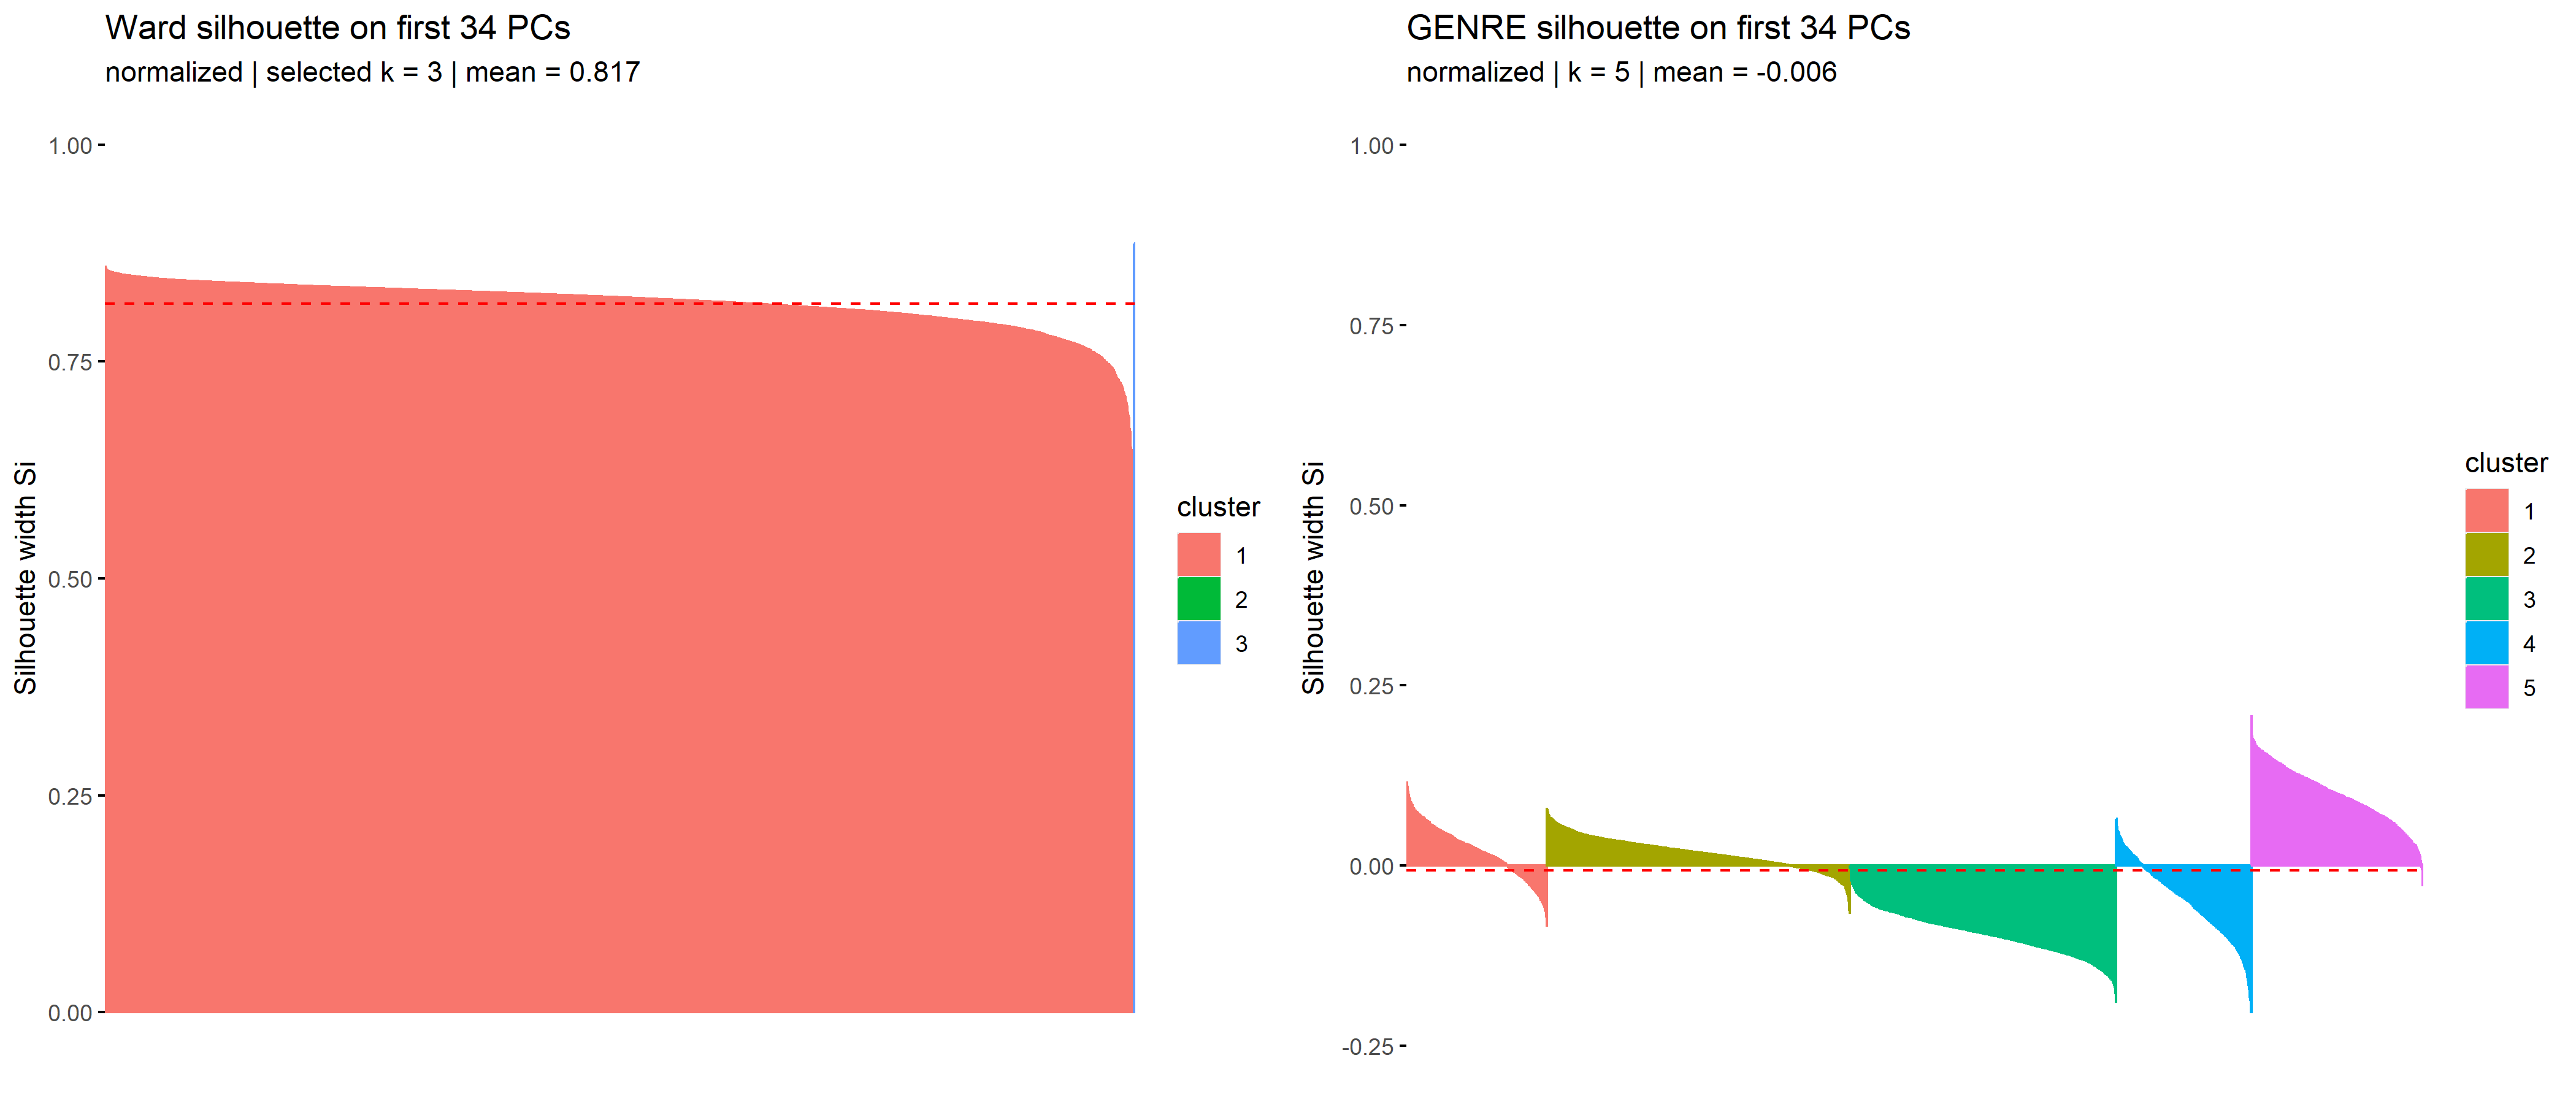
\includegraphics[width=\columnwidth]{../output/part1/hclust_pca/normalized/silhouette_pca_34_components.png}
\caption{Silhouette plots for the normalized PCA scores with \(d=34\) retained components.}
\label{fig:silhouette_normalized_34}
\end{figure}

\subsection{Coefficient Significance in Logistic Regression}
\label{subsec:logistic_significance}
In the binary logistic models of Part II, the significance of each predictor is assessed through the Wald test for an individual regression coefficient \cite{psulogisticwald,rsummaryglm}. If \(\pi(x)=\mathbb{P}(Y=1\mid X=x)\), the fitted model is
\begin{equation}
\log\!\left(\frac{\pi(x)}{1-\pi(x)}\right)=\beta_0+\sum_{j=1}^{p}\beta_j x_j.
\label{eq:logistic_model}
\end{equation}
For each predictor \(x_j\), the implemented null hypothesis is
\begin{equation}
H_0:\beta_j=0.
\label{eq:wald_null}
\end{equation}
Under the large-sample normal approximation for the maximum likelihood estimator,
\begin{equation}
Z_j=\frac{\widehat{\beta}_j}{\mathrm{SE}(\widehat{\beta}_j)} \approx \mathcal{N}(0,1)
\qquad \text{under } H_0,
\label{eq:wald_z}
\end{equation}
or equivalently
\begin{equation}
W_j=Z_j^2=\frac{\widehat{\beta}_j^2}{\mathrm{SE}(\widehat{\beta}_j)^2}\approx \chi^2_1.
\label{eq:wald_chi2}
\end{equation}
Hence the column \texttt{Pr(>|z|)} returned by \texttt{summary(glm(...))} is the two-sided p-value
\begin{equation}
p_j=2\,\mathbb{P}(Z\geq |Z_j|)=2\left[1-\Phi(|Z_j|)\right],
\qquad Z\sim \mathcal{N}(0,1).
\label{eq:wald_pvalue}
\end{equation}
In the present implementation, the reduced model \texttt{Mod1} retains the variables such that \(p_j<0.05\), whereas \texttt{Mod2} retains the variables such that \(p_j<0.20\).

\subsection{Stepwise AIC Selection}
\label{subsec:step_aic}
The model \texttt{ModAIC} of Part II is obtained from the full logistic model \texttt{ModT} by applying \texttt{stepAIC(ModT)} from the \texttt{MASS} package \cite{stepaicmass,raicdoc}. The criterion minimized along the search is Akaike's Information Criterion,
\begin{equation}
\mathrm{AIC}=-2\,\ell(\widehat{\beta})+k\,q,
\label{eq:aic}
\end{equation}
where \(\ell(\widehat{\beta})\) is the maximized log-likelihood of the candidate model, \(q\) is the number of estimated parameters, and \(k=2\) for the classical AIC. Since the code uses \texttt{stepAIC(ModT)} with default arguments, the search starts from the full logistic model and removes terms step by step whenever this decreases the AIC. At each step, among the admissible one-term deletions, the selected move is the one that gives the smallest AIC, and the procedure stops when no further deletion improves the criterion. Formally, if \(\mathcal{M}_0\) is the current model and \(\mathcal{N}(\mathcal{M}_0)\) is the set of candidate one-step submodels explored by the algorithm, the update rule can be summarized as
\begin{equation}
\mathcal{M}_{t+1}=\arg\min_{\mathcal{M}\in\mathcal{N}(\mathcal{M}_t)} \mathrm{AIC}(\mathcal{M}),
\label{eq:stepaic_update}
\end{equation}
provided that this minimum is strictly smaller than \(\mathrm{AIC}(\mathcal{M}_t)\). The resulting model therefore balances fit and parsimony through the AIC penalty rather than through coefficient-wise significance thresholds.

\subsection{Ridge Regularization}
\label{subsec:ridge_regularization}
Following the regularization framework presented in \cite{keribin2025supervised}, the motivation for ridge regression can first be introduced from the classical linear regression setting. In ordinary least squares, the objective is to minimize the residual sum of squares:
\begin{equation}
SCR(\theta)
=
\sum_{i=1}^{n}
\left(
y_i - x_i^\top \theta
\right)^2 .
\label{eq:ols_scr}
\end{equation}
As shown in Equation~\eqref{eq:ols_scr}, the estimator seeks the coefficient vector \(\theta\) that best fits the training data. However, when the number of predictors increases, the model becomes more flexible. This can reduce bias, because the model has greater capacity to adapt to the observed structure, but it can also increase variance, since small perturbations in the training sample may lead to substantially different coefficient estimates.

Ridge regression addresses this issue by replacing the ordinary least-squares criterion with a penalized criterion \cite{keribin2025supervised}:
\begin{equation}
SCR(\theta)
+
\kappa
\sum_{j=1}^{p}
\theta_j^2 .
\label{eq:ridge_penalized_criterion}
\end{equation}

Equivalently, the ridge estimator is defined as
\begin{equation}
\widehat{\theta}_{\mathrm{ridge}}
=
\arg\min_{\theta}
\left[
\sum_{i=1}^{n}
\left(
y_i - x_i^\top \theta
\right)^2
+
\kappa
\sum_{j=1}^{p}
\theta_j^2
\right].
\label{eq:ridge_estimator}
\end{equation}

In Equations~\eqref{eq:ridge_penalized_criterion} and~\eqref{eq:ridge_estimator}, the term
\begin{equation}
\kappa
\sum_{j=1}^{p}
\theta_j^2
\label{eq:ridge_penalty}
\end{equation}
penalizes excessively large coefficients. The parameter \(\kappa \geq 0\) controls the strength of the regularization. When \(\kappa = 0\), the non-regularized estimator is recovered. As \(\kappa\) increases, the penalty becomes stronger and the estimated coefficients are progressively shrunk toward zero.

From the perspective of the bias--variance trade-off, ridge regularization introduces additional bias in order to reduce the variance of the estimator. This is particularly relevant in the presence of correlated predictors, because ridge tends to distribute the effect more smoothly among related variables instead of producing unstable coefficient estimates. Therefore, ridge is not primarily used for variable selection, but rather to stabilize the estimation process, control the effective complexity of the model, and improve generalization performance.

In the logistic regression context considered in this project, the same regularization principle is applied by penalizing the negative log-likelihood. If \(\ell(\beta)\) denotes the log-likelihood of the logistic model, the ridge logistic estimator is obtained by solving
\begin{equation}
\widehat{\beta}_{\mathrm{ridge}}
=
\arg\min_{\beta}
\left[
-\ell(\beta)
+
\kappa
\sum_{j=1}^{p}
\beta_j^2
\right].
\label{eq:ridge_logistic_estimator}
\end{equation}
Thus, Equation~\eqref{eq:ridge_logistic_estimator} extends the ridge principle described in \cite{keribin2025supervised} to the binary classification problem. In this setting, the regularization term reduces the magnitude of the logistic regression coefficients, improves numerical stability, and limits overfitting when the predictor space is high-dimensional.

\begin{figure}[H]
\centering
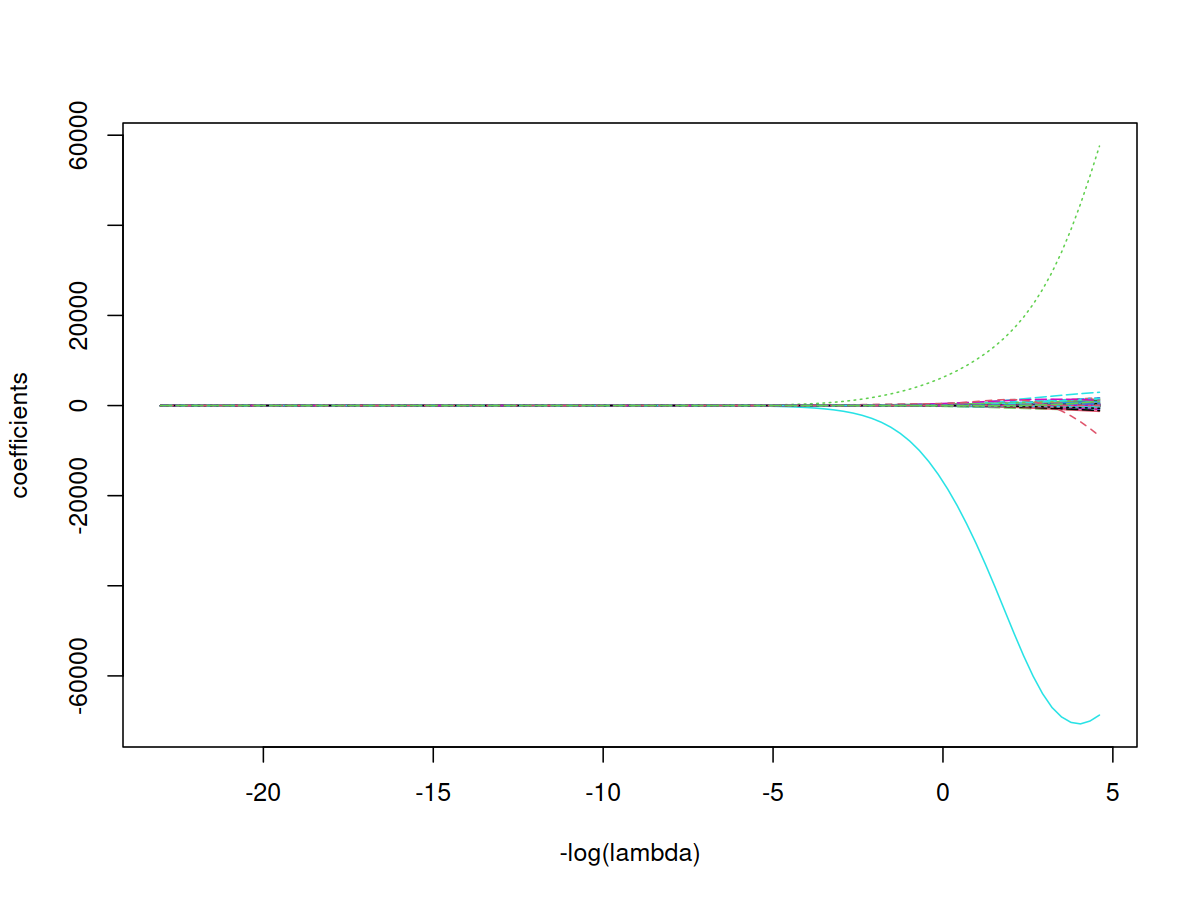
\includegraphics[width=\columnwidth]{../output/part2/ridge/ridge_coefficients_loglambda.png}
\caption{Ridge coefficient paths as functions of \(-\log(\lambda)\). Moving to the right corresponds to weaker penalization and larger coefficient magnitudes.}
\label{fig:ridge_coefficients_loglambda}
\end{figure}
